
%% bare_jrnl.tex
%% V1.3
%% 2007/01/11
%% by Michael Shell
%% see http://www.michaelshell.org/
%% for current contact information.
%%
%% This is a skeleton file demonstrating the use of IEEEtran.cls
%% (requires IEEEtran.cls version 1.7 or later) with an IEEE journal paper.
%%
%% Support sites:
%% http://www.michaelshell.org/tex/ieeetran/
%% http://www.ctan.org/tex-archive/macros/latex/contrib/IEEEtran/
%% and
%% http://www.ieee.org/



% *** Authors should verify (and, if needed, correct) their LaTeX system  ***
% *** with the testflow diagnostic prior to trusting their LaTeX platform ***
% *** with production work. IEEE's font choices can trigger bugs that do  ***
% *** not appear when using other class files.                            ***
% The testflow support page is at:
% http://www.michaelshell.org/tex/testflow/


%%*************************************************************************
%% Legal Notice:
%% This code is offered as-is without any warranty either expressed or
%% implied; without even the implied warranty of MERCHANTABILITY or
%% FITNESS FOR A PARTICULAR PURPOSE!
%% User assumes all risk.
%% In no event shall IEEE or any contributor to this code be liable for
%% any damages or losses, including, but not limited to, incidental,
%% consequential, or any other damages, resulting from the use or misuse
%% of any information contained here.
%%
%% All comments are the opinions of their respective authors and are not
%% necessarily endorsed by the IEEE.
%%
%% This work is distributed under the LaTeX Project Public License (LPPL)
%% ( http://www.latex-project.org/ ) version 1.3, and may be freely used,
%% distributed and modified. A copy of the LPPL, version 1.3, is included
%% in the base LaTeX documentation of all distributions of LaTeX released
%% 2003/12/01 or later.
%% Retain all contribution notices and credits.
%% ** Modified files should be clearly indicated as such, including  **
%% ** renaming them and changing author support contact information. **
%%
%% File list of work: IEEEtran.cls, IEEEtran_HOWTO.pdf, bare_adv.tex,
%%                    bare_conf.tex, bare_jrnl.tex, bare_jrnl_compsoc.tex
%%*************************************************************************

% Note that the a4paper option is mainly intended so that authors in
% countries using A4 can easily print to A4 and see how their papers will
% look in print - the typesetting of the document will not typically be
% affected with changes in paper size (but the bottom and side margins will).
% Use the testflow package mentioned above to verify correct handling of
% both paper sizes by the user's LaTeX system.
%
% Also note that the "draftcls" or "draftclsnofoot", not "draft", option
% should be used if it is desired that the figures are to be displayed in
% draft mode.
%
\documentclass[journal]{IEEEtran}
%
% If IEEEtran.cls has not been installed into the LaTeX system files,
% manually specify the path to it like:
% \documentclass[journal]{../sty/IEEEtran}





% Some very useful LaTeX packages include:
% (uncomment the ones you want to load)


% *** MISC UTILITY PACKAGES ***
%
%\usepackage{ifpdf}
% Heiko Oberdiek's ifpdf.sty is very useful if you need conditional
% compilation based on whether the output is pdf or dvi.
% usage:
% \ifpdf
%   % pdf code
% \else
%   % dvi code
% \fi
% The latest version of ifpdf.sty can be obtained from:
% http://www.ctan.org/tex-archive/macros/latex/contrib/oberdiek/
% Also, note that IEEEtran.cls V1.7 and later provides a builtin
% \ifCLASSINFOpdf conditional that works the same way.
% When switching from latex to pdflatex and vice-versa, the compiler may
% have to be run twice to clear warning/error messages.






% *** CITATION PACKAGES ***
%
\usepackage{cite}
% cite.sty was written by Donald Arseneau
% V1.6 and later of IEEEtran pre-defines the format of the cite.sty package
% \cite{} output to follow that of IEEE. Loading the cite package will
% result in citation numbers being automatically sorted and properly
% "compressed/ranged". e.g., [1], [9], [2], [7], [5], [6] without using
% cite.sty will become [1], [2], [5]--[7], [9] using cite.sty. cite.sty's
% \cite will automatically add leading space, if needed. Use cite.sty's
% noadjust option (cite.sty V3.8 and later) if you want to turn this off.
% cite.sty is already installed on most LaTeX systems. Be sure and use
% version 4.0 (2003-05-27) and later if using hyperref.sty. cite.sty does
% not currently provide for hyperlinked citations.
% The latest version can be obtained at:
% http://www.ctan.org/tex-archive/macros/latex/contrib/cite/
% The documentation is contained in the cite.sty file itself.






% *** GRAPHICS RELATED PACKAGES ***
%
\ifCLASSINFOpdf
   \usepackage[pdftex]{graphicx}
  % declare the path(s) where your graphic files are
  % \graphicspath{{../pdf/}{../jpeg/}}
  % and their extensions so you won't have to specify these with
  % every instance of \includegraphics
  % \DeclareGraphicsExtensions{.pdf,.jpeg,.png}
\else
  % or other class option (dvipsone, dvipdf, if not using dvips). graphicx
  % will default to the driver specified in the system graphics.cfg if no
  % driver is specified.
   \usepackage[dvips]{graphicx}
  % declare the path(s) where your graphic files are
  % \graphicspath{{../eps/}}
  % and their extensions so you won't have to specify these with
  % every instance of \includegraphics
  % \DeclareGraphicsExtensions{.eps}
\fi
% graphicx was written by David Carlisle and Sebastian Rahtz. It is
% required if you want graphics, photos, etc. graphicx.sty is already
% installed on most LaTeX systems. The latest version and documentation can
% be obtained at:
% http://www.ctan.org/tex-archive/macros/latex/required/graphics/
% Another good source of documentation is "Using Imported Graphics in
% LaTeX2e" by Keith Reckdahl which can be found as epslatex.ps or
% epslatex.pdf at: http://www.ctan.org/tex-archive/info/
%
% latex, and pdflatex in dvi mode, support graphics in encapsulated
% postscript (.eps) format. pdflatex in pdf mode supports graphics
% in .pdf, .jpeg, .png and .mps (metapost) formats. Users should ensure
% that all non-photo figures use a vector format (.eps, .pdf, .mps) and
% not a bitmapped formats (.jpeg, .png). IEEE frowns on bitmapped formats
% which can result in "jaggedy"/blurry rendering of lines and letters as
% well as large increases in file sizes.
%
% You can find documentation about the pdfTeX application at:
% http://www.tug.org/applications/pdftex





% *** MATH PACKAGES ***
%
\usepackage[cmex10]{amsmath}
\usepackage{amssymb}
% A popular package from the American Mathematical Society that provides
% many useful and powerful commands for dealing with mathematics. If using
% it, be sure to load this package with the cmex10 option to ensure that
% only type 1 fonts will utilized at all point sizes. Without this option,
% it is possible that some math symbols, particularly those within
% footnotes, will be rendered in bitmap form which will result in a
% document that can not be IEEE Xplore compliant!
%
% Also, note that the amsmath package sets \interdisplaylinepenalty to 10000
% thus preventing page breaks from occurring within multiline equations. Use:
%\interdisplaylinepenalty=2500
% after loading amsmath to restore such page breaks as IEEEtran.cls normally
% does. amsmath.sty is already installed on most LaTeX systems. The latest
% version and documentation can be obtained at:
% http://www.ctan.org/tex-archive/macros/latex/required/amslatex/math/



\usepackage{algorithm}
\usepackage{algorithmic}


% *** SPECIALIZED LIST PACKAGES ***
%
%\usepackage{algorithmic}
% algorithmic.sty was written by Peter Williams and Rogerio Brito.
% This package provides an algorithmic environment fo describing algorithms.
% You can use the algorithmic environment in-text or within a figure
% environment to provide for a floating algorithm. Do NOT use the algorithm
% floating environment provided by algorithm.sty (by the same authors) or
% algorithm2e.sty (by Christophe Fiorio) as IEEE does not use dedicated
% algorithm float types and packages that provide these will not provide
% correct IEEE style captions. The latest version and documentation of
% algorithmic.sty can be obtained at:
% http://www.ctan.org/tex-archive/macros/latex/contrib/algorithms/
% There is also a support site at:
% http://algorithms.berlios.de/index.html
% Also of interest may be the (relatively newer and more customizable)
% algorithmicx.sty package by Szasz Janos:
% http://www.ctan.org/tex-archive/macros/latex/contrib/algorithmicx/




% *** ALIGNMENT PACKAGES ***
%
%\usepackage{array}
% Frank Mittelbach's and David Carlisle's array.sty patches and improves
% the standard LaTeX2e array and tabular environments to provide better
% appearance and additional user controls. As the default LaTeX2e table
% generation code is lacking to the point of almost being broken with
% respect to the quality of the end results, all users are strongly
% advised to use an enhanced (at the very least that provided by array.sty)
% set of table tools. array.sty is already installed on most systems. The
% latest version and documentation can be obtained at:
% http://www.ctan.org/tex-archive/macros/latex/required/tools/


%\usepackage{mdwmath}
%\usepackage{mdwtab}
% Also highly recommended is Mark Wooding's extremely powerful MDW tools,
% especially mdwmath.sty and mdwtab.sty which are used to format equations
% and tables, respectively. The MDWtools set is already installed on most
% LaTeX systems. The lastest version and documentation is available at:
% http://www.ctan.org/tex-archive/macros/latex/contrib/mdwtools/


% IEEEtran contains the IEEEeqnarray family of commands that can be used to
% generate multiline equations as well as matrices, tables, etc., of high
% quality.


%\usepackage{eqparbox}
% Also of notable interest is Scott Pakin's eqparbox package for creating
% (automatically sized) equal width boxes - aka "natural width parboxes".
% Available at:
% http://www.ctan.org/tex-archive/macros/latex/contrib/eqparbox/





% *** SUBFIGURE PACKAGES ***
%\usepackage[tight,footnotesize]{subfigure}
% subfigure.sty was written by Steven Douglas Cochran. This package makes it
% easy to put subfigures in your figures. e.g., "Figure 1a and 1b". For IEEE
% work, it is a good idea to load it with the tight package option to reduce
% the amount of white space around the subfigures. subfigure.sty is already
% installed on most LaTeX systems. The latest version and documentation can
% be obtained at:
% http://www.ctan.org/tex-archive/obsolete/macros/latex/contrib/subfigure/
% subfigure.sty has been superceeded by subfig.sty.



%\usepackage[caption=false]{caption}
%\usepackage[font=footnotesize]{subfig}
% subfig.sty, also written by Steven Douglas Cochran, is the modern
% replacement for subfigure.sty. However, subfig.sty requires and
% automatically loads Axel Sommerfeldt's caption.sty which will override
% IEEEtran.cls handling of captions and this will result in nonIEEE style
% figure/table captions. To prevent this problem, be sure and preload
% caption.sty with its "caption=false" package option. This is will preserve
% IEEEtran.cls handing of captions. Version 1.3 (2005/06/28) and later
% (recommended due to many improvements over 1.2) of subfig.sty supports
% the caption=false option directly:
%\usepackage[caption=false,font=footnotesize]{subfig}
%
% The latest version and documentation can be obtained at:
% http://www.ctan.org/tex-archive/macros/latex/contrib/subfig/
% The latest version and documentation of caption.sty can be obtained at:
% http://www.ctan.org/tex-archive/macros/latex/contrib/caption/




% *** FLOAT PACKAGES ***
%
%\usepackage{fixltx2e}
% fixltx2e, the successor to the earlier fix2col.sty, was written by
% Frank Mittelbach and David Carlisle. This package corrects a few problems
% in the LaTeX2e kernel, the most notable of which is that in current
% LaTeX2e releases, the ordering of single and double column floats is not
% guaranteed to be preserved. Thus, an unpatched LaTeX2e can allow a
% single column figure to be placed prior to an earlier double column
% figure. The latest version and documentation can be found at:
% http://www.ctan.org/tex-archive/macros/latex/base/



%\usepackage{stfloats}
% stfloats.sty was written by Sigitas Tolusis. This package gives LaTeX2e
% the ability to do double column floats at the bottom of the page as well
% as the top. (e.g., "\begin{figure*}[!b]" is not normally possible in
% LaTeX2e). It also provides a command:
%\fnbelowfloat
% to enable the placement of footnotes below bottom floats (the standard
% LaTeX2e kernel puts them above bottom floats). This is an invasive package
% which rewrites many portions of the LaTeX2e float routines. It may not work
% with other packages that modify the LaTeX2e float routines. The latest
% version and documentation can be obtained at:
% http://www.ctan.org/tex-archive/macros/latex/contrib/sttools/
% Documentation is contained in the stfloats.sty comments as well as in the
% presfull.pdf file. Do not use the stfloats baselinefloat ability as IEEE
% does not allow \baselineskip to stretch. Authors submitting work to the
% IEEE should note that IEEE rarely uses double column equations and
% that authors should try to avoid such use. Do not be tempted to use the
% cuted.sty or midfloat.sty packages (also by Sigitas Tolusis) as IEEE does
% not format its papers in such ways.


%\ifCLASSOPTIONcaptionsoff
%  \usepackage[nomarkers]{endfloat}
% \let\MYoriglatexcaption\caption
% \renewcommand{\caption}[2][\relax]{\MYoriglatexcaption[#2]{#2}}
%\fi
% endfloat.sty was written by James Darrell McCauley and Jeff Goldberg.
% This package may be useful when used in conjunction with IEEEtran.cls'
% captionsoff option. Some IEEE journals/societies require that submissions
% have lists of figures/tables at the end of the paper and that
% figures/tables without any captions are placed on a page by themselves at
% the end of the document. If needed, the draftcls IEEEtran class option or
% \CLASSINPUTbaselinestretch interface can be used to increase the line
% spacing as well. Be sure and use the nomarkers option of endfloat to
% prevent endfloat from "marking" where the figures would have been placed
% in the text. The two hack lines of code above are a slight modification of
% that suggested by in the endfloat docs (section 8.3.1) to ensure that
% the full captions always appear in the list of figures/tables - even if
% the user used the short optional argument of \caption[]{}.
% IEEE papers do not typically make use of \caption[]'s optional argument,
% so this should not be an issue. A similar trick can be used to disable
% captions of packages such as subfig.sty that lack options to turn off
% the subcaptions:
% For subfig.sty:
% \let\MYorigsubfloat\subfloat
% \renewcommand{\subfloat}[2][\relax]{\MYorigsubfloat[]{#2}}
% For subfigure.sty:
% \let\MYorigsubfigure\subfigure
% \renewcommand{\subfigure}[2][\relax]{\MYorigsubfigure[]{#2}}
% However, the above trick will not work if both optional arguments of
% the \subfloat/subfig command are used. Furthermore, there needs to be a
% description of each subfigure *somewhere* and endfloat does not add
% subfigure captions to its list of figures. Thus, the best approach is to
% avoid the use of subfigure captions (many IEEE journals avoid them anyway)
% and instead reference/explain all the subfigures within the main caption.
% The latest version of endfloat.sty and its documentation can obtained at:
% http://www.ctan.org/tex-archive/macros/latex/contrib/endfloat/
%
% The IEEEtran \ifCLASSOPTIONcaptionsoff conditional can also be used
% later in the document, say, to conditionally put the References on a
% page by themselves.





% *** PDF, URL AND HYPERLINK PACKAGES ***
%
\usepackage{url}
% url.sty was written by Donald Arseneau. It provides better support for
% handling and breaking URLs. url.sty is already installed on most LaTeX
% systems. The latest version can be obtained at:
% http://www.ctan.org/tex-archive/macros/latex/contrib/misc/
% Read the url.sty source comments for usage information. Basically,
% \url{my_url_here}.


\usepackage[all]{xy}


% *** Do not adjust lengths that control margins, column widths, etc. ***
% *** Do not use packages that alter fonts (such as pslatex).         ***
% There should be no need to do such things with IEEEtran.cls V1.6 and later.
% (Unless specifically asked to do so by the journal or conference you plan
% to submit to, of course. )


% correct bad hyphenation here
\hyphenation{op-tical net-works semi-conduc-tor}

\makeatletter
\newcommand{\rmnum}[1]{\romannumeral #1}
\newcommand{\Rmnum}[1]{\expandafter\@slowromancap\romannumeral #1@}
\makeatother

\begin{document}
%
% paper title
% can use linebreaks \\ within to get better formatting as desired
\title{A Halting Algorithm to Determine the Existence of the Decoder}
%
%
% author names and IEEE memberships
% note positions of commas and nonbreaking spaces ( ~ ) LaTeX will not break
% a structure at a ~ so this keeps an author's name from being broken across
% two lines.
% use \thanks{} to gain access to the first footnote area
% a separate \thanks must be used for each paragraph as LaTeX2e's \thanks
% was not built to handle multiple paragraphs
%

%\author{Michael~Shell,~\IEEEmembership{Member,~IEEE,}
%        John~Doe,~\IEEEmembership{Fellow,~OSA,}
%        and~Jane~Doe,~\IEEEmembership{Life~Fellow,~IEEE}% <-this % stops a space
%\thanks{M. Shell is with the Department
%of Electrical and Computer Engineering, Georgia Institute of Technology, Atlanta,
%GA, 30332 USA e-mail: (see http://www.michaelshell.org/contact.html).}% <-this % stops a space
%\thanks{J. Doe and J. Doe are with Anonymous University.}% <-this % stops a space
%\thanks{Manuscript received April 19, 2005; revised January 11, 2007.}}
\author{ShengYu~Shen,~\IEEEmembership{Member,~IEEE,}
        Ying~Qin,
        LiQuan~Xiao,
        KeFei~Wang,
        JianMin~Zhang,
        and~SiKun~Li% <-this % stops a space
\thanks{The authors are with the School of Computer,
National University of Defense Technology, ChangSha,
HuNan, 410073 CHINA. e-mail: \{syshen, qy123, lqxiao, kfwang, jmzhang, skli\}@nudt.edu.cn, (see http://www.ssypub.org/).}% <-this % stops a space
%\thanks{Manuscript received September 18, 2009; revised January 10, 2010.
%The work of ShengYu Shen was fund by project 60603088 supported by National Natural Science Foundation of China,
%and also fund by the Program for Changjiang
%Scholars and Innovative Research Team in University No
%IRT0614.
%This paper was recommended by Associate Editor Steven Nowick.}
%\thanks{Copyright (c) 2010 IEEE. Personal use of this material is
%permitted. However, permission to use this material
%for any other purposes must be obtained from the IEEE by
%sending an email to pubs-permissions@ieee.org.}
}
% note the % following the last \IEEEmembership and also \thanks -
% these prevent an unwanted space from occurring between the last author name
% and the end of the author line. i.e., if you had this:
%
% \author{....lastname \thanks{...} \thanks{...} }
%                     ^------------^------------^----Do not want these spaces!
%
% a space would be appended to the last name and could cause every name on that
% line to be shifted left slightly. This is one of those "LaTeX things". For
% instance, "\textbf{A} \textbf{B}" will typeset as "A B" not "AB". To get
% "AB" then you have to do: "\textbf{A}\textbf{B}"
% \thanks is no different in this regard, so shield the last } of each \thanks
% that ends a line with a % and do not let a space in before the next \thanks.
% Spaces after \IEEEmembership other than the last one are OK (and needed) as
% you are supposed to have spaces between the names. For what it is worth,
% this is a minor point as most people would not even notice if the said evil
% space somehow managed to creep in.



% The paper headers
\markboth{IEEE Transactions on COMPUTER-AIDED DESIGN of Integrated Circuits and Systems ,~Vol.~x, No.~x, xx~20xx}%
{Shell \MakeLowercase{\textit{et al.}}: Bare Demo of IEEEtran.cls for Journals}
% The only time the second header will appear is for the odd numbered pages
% after the title page when using the twoside option.
%
% *** Note that you probably will NOT want to include the author's ***
% *** name in the headers of peer review papers.                   ***
% You can use \ifCLASSOPTIONpeerreview for conditional compilation here if
% you desire.




% If you want to put a publisher's ID mark on the page you can do it like
% this:
%\IEEEpubid{0000--0000/00\$00.00~\copyright~2007 IEEE}
% Remember, if you use this you must call \IEEEpubidadjcol in the second
% column for its text to clear the IEEEpubid mark.



% use for special paper notices
%\IEEEspecialpapernotice{(Invited Paper)}




% make the title area
\maketitle


\begin{abstract}
Complementary synthesis automatically synthesizes the decoder circuit of an encoder.
It determines the existence of the decoder by checking whether the encoder's input can be uniquely determined by its output.
However,
this algorithm will not halt if the decoder does not exist.

To solve this problem,
a novel halting algorithm is proposed.
For every state sequence of the encoder,
this algorithm first checks whether the encoder's input can be uniquely determined by its output.
If yes,
the decoder exists;
Otherwise,
this algorithm checks that if this state sequence contains loops,
which can be further expanded to prove the non-existence of the decoder for all those longer state sequences.

To illustrate its usefulness and efficiency,
this algorithm has been run on several complex encoders,
including PCI-E and Ethernet.
Experimental results indicate that
this algorithm always halts properly by distinguishing correct encoders from the incorrect ones,
and it can be more than three times faster than the previous work.
\end{abstract}
% IEEEtran.cls defaults to using nonbold math in the Abstract.
% This preserves the distinction between vectors and scalars. However,
% if the journal you are submitting to favors bold math in the abstract,
% then you can use LaTeX's standard command \boldmath at the very start
% of the abstract to achieve this. Many IEEE journals frown on math
% in the abstract anyway.

% Note that keywords are not normally used for peerreview papers.
\begin{IEEEkeywords}
Halting Algorithm, Complementary Synthesis
\end{IEEEkeywords}






% For peer review papers, you can put extra information on the cover
% page as needed:
% \ifCLASSOPTIONpeerreview
% \begin{center} \bfseries EDICS Category: 3-BBND \end{center}
% \fi
%
% For peerreview papers, this IEEEtran command inserts a page break and
% creates the second title. It will be ignored for other modes.
\IEEEpeerreviewmaketitle


\newtheorem{algo}{\textbf{Algorithm}}
\newtheorem{definition11}{\textbf{Definition}}
\newtheorem{lemma}{\textbf{Lemma}}
\newtheorem{theorem}{\textbf{Theorem}}
\newtheorem{proposition}{\textbf{Proposition}}

\section{Introduction}\label{sec_intro}
\textbf{One of the most difficult jobs in designing communication and multimedia chips
is to design and verify the complex complementary circuit pair $(E,E^{-1})$,
in which the encoder $E$ transforms information into a format suitable for transmission and storage,
while its complementary circuit(or decoder) $E^{-1}$ recovers this information.
In order to facilitate this job,
the complementary synthesis algorithm is proposed in \cite{ShengYuShen:iccad09,ShengYuShen:tcad}
to automatically synthesize the decoder circuit of an encoder,
by checking the Parameterized Complementary Condition(PC),
that is,
whether the encoder's input letter can be uniquely determined by its output sequence.}

However,
that algorithm will not halt if $E^{-1}$ does not exist.
Another algorithm has been proposed in \cite{ShengYuShen:fmcad10} to solve this problem
by first constructing a list of over-approximations of PC that is similar to onion rings,
and then checking whether $E$ is in all these rings.
This algorithm is very slow and complicated.
Therefore yet another halting algorithm is proposed in this paper,
which is both faster and more straightforward.
\textbf{For every state sequence of the encoder,
this new algorithm checks two cases:}

\begin{enumerate}
 \item \textbf{Just like the non-halting algorithm\cite{ShengYuShen:iccad09,ShengYuShen:tcad},
       checking whether the encoder's input can be uniquely determined by its output.
      If yes, the decoder exists;}
 \item \textbf{Otherwise,
       checking whether there are loops in the state sequence mentioned above.
       As shown in Figure \ref{doubleloop_unfold_cmp_simple},
       the state sequence in Figure \ref{doubleloop_unfold_cmp_simple}a) contains three sub-sequences $a$, $b$ and $c$.
       The sub-sequence $b$ is a loop
       that can be further expanded to obtain a longer state sequence shown in Figure \ref{doubleloop_unfold_cmp_simple}b).
       In this way,
       the non-existence of the decoder can be proved for all those longer state sequences.}
\end{enumerate}

\begin{figure}[b]
\begin{center}
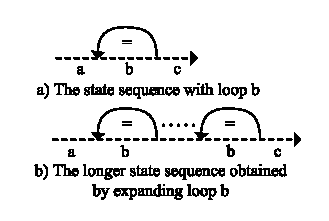
\includegraphics[width=0.3\textwidth]{doubleloop_unfold_cmp_simple}
\end{center}
\caption{Expanding the loop to prove the non-existence of the decoder for longer state sequence}
  \label{doubleloop_unfold_cmp_simple}
\end{figure}

This new algorithm has been implemented with the OCaml language.
All generated SAT instances are solved with Zchaff SAT solver\cite{CHAFF}.
The benchmark set includes several complex encoders from industrial projects
(e.g.,
PCI-E\cite{PCIESPEC} and Ethernet\cite{IEEE80232002}),
and their slightly modified variants without corresponding decoders.
Experimental results indicate that
this paper's algorithm always halts properly by distinguishing correct encoders from incorrect ones,
and can be three times faster than the other halting algorithm\cite{ShengYuShen:fmcad10} proposed by us in FMCAD'10.
All these experimental results and programs can be downloaded from \url{http://www.ssypub.org}.

\textbf{There is one more issue that needs to be clarified.
There are two classes of complementary circuit pairs with different characters and design methodologies:}
\begin{enumerate}
  \item \textbf{Standard datapath-intensive circuits:
  These circuits often work as digital signal processing components, such as
      Fast Fourier Transform (FFT) and
      Discrete Cosine Transform(DCT).
      These circuits usually have standard and highly optimized implementations from various foundries and IP vendors,
      such as Xilinx core generator\cite{CoreGen} and Synopsys DesignWare library\cite{DesignWare}.
      Therefore this paper's algorithm isn't design for them.}
  \item \textbf{Non-standard and control-intensive circuits:
  These circuits,
  such as PCI-E\cite{PCIESPEC} and Ethernet\cite{IEEE80232002},
  are often used to handle communication protocols,
  and typically don't have standard implementations.
      This paper's algorithm is designed for them.}
\end{enumerate}


\textbf{The remainder of this paper is organized as follows}.
Section \ref{sec_prem} presents background materials.
Section \ref{sec_exist} introduces this paper's algorithm,
while Section \ref{sec_rmred} describes how to remove redundant output letters to minimize the circuit area.
Section \ref{sec_exp} and \ref{sec_relwork} present the experimental results and related works respectively.
Finally,
Section \ref{sec_conclude} concludes this paper.

\section{Preliminaries}\label{sec_prem}


\subsection{Propositional Satisfiability}\label{subsec_SAT}
The Boolean value set is denoted as $B=\{0,1\}$.
For a Boolean formula $F$ over a variable set $V$,
the propositional satisfiability problem(abbreviated as SAT) is to find a satisfying assignment $A:V\to B$,
so that $F$ can be evaluated to 1.
If such a satisfying assignment exists, then $F$ is satisfiable;
otherwise,
it is unsatisfiable.

A computer program that decides the existence of such a satisfying assignment is called a SAT solver,
such as Zchaff\cite{CHAFF}, Grasp\cite{grasp}, Berkmin\cite{BERKMIN},
and MiniSAT\cite{EXTSAT}.
A formula to be solved by a SAT solver is also called a SAT instance.

%Normally,
%a SAT solver requires formula $F$ to be represented in the \textbf{Conjunctive Normal Form(CNF)} or the \textbf{And-Inverter Graph(AIG)} formats.
%In this paper we will only discuss the CNF format,
%in which a \textbf{formula} $F=\bigwedge_{cl\in CL}cl$ is a conjunction of its clause set $CL$,
%and a \textbf{clause} $cl=\bigvee_{l\in Lit}l$ is a disjunction of its literal set $Lit$,
%and a \textbf{literal} is a variable $v$ or its negation $\neg v$.
%A formula in the CNF format is also called a \textbf{SAT instance}.
%
%\begin{definition11}\label{resolution}
%\textbf{Resolution}: For clause $c=l_1\vee\dots\vee l_n$ and $c'=l'_1\vee\dots\vee l'_m$,
%assume that for a particular variable $v$,
%there are two indices $0\le i\le n$ and $0\le j\le m$,
%such that $l_i\equiv v$ and $l'_j\equiv \neg v$,
%then resolution of $c$ and $c'$ is :
%\begin{displaymath}
%resolve(c,c')=\{l_p|p\ne i\}\cup \{l'_p|p\ne j\}
%\end{displaymath}
%and $v$ is the pivot variable of $c$ and $c'$.
%\end{definition11}

%An unsatisfiable formula often has many clause subsets that are also unsatisfiable,
%these subsets are called \textbf{unsatisfiable cores}.
%Some unsatisfiable core extraction algorithms are proposed by Goldberg et al.\cite{VERPROOF} and Zhang et al.\cite{VALIDSAT}.



\subsection{Recurrence Diameter}\label{subsec_recdia}

The encoder $E$ can be modeled by a Mealy finite state machine \cite{MEALY}.

\begin{definition11}\label{MealyFSM}%\addtolength{\itemsep}{-0.5\baselineskip}
%{\setlength{\baselineskip}{0.5\baselineskip}
\textbf{Mealy finite state machine} is a 5-tuple $M=(S,s_0,I,O,T)$,
consisting of a finite state set $S$,
an initial state $s_0\in S$,
a finite set of input letters $I$,
a finite set of output letters $O$,
a transition function $T: S\times I\to S\times O$ that computes the next state and the output letter from the current state and the input letter.
%}
\end{definition11}
\begin{figure}[t]
\begin{center}
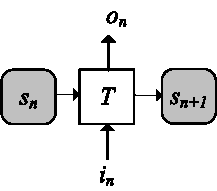
\includegraphics[width=0.20\textwidth]{mealy}
\end{center}
\caption{Mealy finite state machine}
  \label{mealy}
\end{figure}

As shown in Figure \ref{mealy},
as well as in the remainder of this paper,
the state is represented as a gray round corner box,
and the transition function $T$ is represented by a white rectangle.
The state, the input letter and the output letter at the $n$-th cycle are denoted as $s_n$, $i_n$ and $o_n$ respectively.
The sequence of state, input letter and output letter from the $n$-th to the $m$-th cycle are denoted as $s_n^m$, $i_n^m$ and $o_n^m$ respectively.
\textbf{A loop is a state sequence $s_n^{m}$ with $s_n\equiv s_m$.
A loop-like path is a state sequence $s_n^{m}$ with $s_i\equiv s_j$,
where $n\le i< j\le m$.}


Kroening et al. \cite{RecDiam} defined the \textbf{state variables recurrence diameter} of $M$,
denoted by $rrd(M)$,
as the longest state sequence that starts from an initial state and does not contain a loop.

\begin{equation}\label{equ_svrd}
\begin{split}
&rrd(M)\overset{def}{=}\max\{i|\exists s_0 \dots s_i i_0 \dots i_i o_0 \dots o_i:\\
& I(s_0)\wedge \bigwedge^{i-1}_{j=0}(s_{j+1},o_j)\equiv T(s_j,i_j)\wedge\bigwedge^{i-1}_{j=0}\bigwedge^{i}_{k=j+1}s_{j}\ne s_{k}\}
\end{split}
\end{equation}

In this paper,
a similar concept: the \textbf{uninitialized state variables recurrence diameter} of $M$,
denoted by $uirrd(M)$,
is defined as the longest state sequence without loop.
%}

\begin{equation}\label{equ_uisvrd}
\begin{split}
&uirrd(M)\overset{def}{=}\max\{i|\exists s_0 \dots s_i i_0 \dots i_i o_0 \dots o_i:\\
&\bigwedge^{i-1}_{j=0}(s_{j+1},o_j)\equiv T(s_j,i_j)\wedge\bigwedge^{i-1}_{j=0}\bigwedge^{i}_{k=j+1}s_{j}\ne s_{k}\}
\end{split}
\end{equation}

The only difference between these two definitions is that $uirrd$ does not consider the initial state.
\textbf{These definitions are only used in proving the theorems below.
This paper's algorithm does not need to compute these diameters.}

\subsection{The Original Non-halting Algorithm to Determine the Existence of the Decoder}\label{subsec_chkextdec}
The complementary synthesis algorithm\cite{ShengYuShen:iccad09} includes two steps:
determining the existence of the decoder and characterizing its Boolean function.
Only the first step is introduced here.

\textbf{According to our previous research \cite{ShengYuShen:iccad09,ShengYuShen:tcad,ShengYuShen:fmcad10},
and our engineering experience in designing communication chips for the TH-1A supercomputer\cite{TH1A},
many communication protocols are lossless,
that is,
every input letter can be recovered from its output sequence.}

More formally,
as shown in Figure \ref{t1},
a sufficient condition for the existence of the decoder $E^{-1}$ is,
there exist three parameter values $p$, $d$ and $l$,
so that $i_n$ of the encoder $E$ can be uniquely determined by $E$'s output sequence $o_{n+d-l}^{n+d-1}$.
$d$ is the relative delay between $o_{n+d-l}^{n+d-1}$ and the input letter $i_n$,
while $l$ is the length of $o_{n+d-l}^{n+d-1}$,
and $p$ is the length of the prefix state sequence used to rule out some unreachable states of the encoder.
Thus,
the parameterized complementary condition($PC$)\cite{ShengYuShen:iccad09} can be formally defined  as:

\begin{figure}[t]
\begin{center}
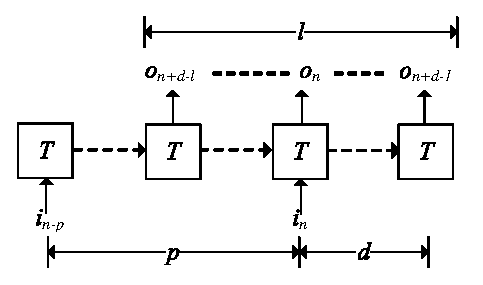
\includegraphics[width=0.4\textwidth]{t1}
\end{center}
\caption{The parameterized complementary condition}
  \label{t1}
\end{figure}

%However,
%the unique condition is unnecessarily restrictive,
%because it may not hold when $s_n$ is not reachable,
%even if $E$ is a correct encoder whose input can be uniquely determined by its output in its reachable state set.
%So we need to rule out unreachable states before checking the unique condition.
%
%The continuous running character of communication circuits provides us an opportunity to rule out unreachable states easily without paying the expensive cost of computing the reachable state set.
%That is to say,
%we only need to check the unique condition on the state set $RS^{\infty}$ that can be reached infinitely often from $S$.
%
%\begin{equation}
%RS^{q}\overset{def}{=} \{s_q|\bigwedge_{m=0}^{q-1}\{(s_{m+1},o_m)\equiv T(s_m,i_m)\}\}
%\end{equation}
%\begin{equation}
%RS^{>p}\overset{def}{=}\bigcup_{q>p} RS^{q}
%\end{equation}
%\begin{equation}\label{rse}
%RS^{\infty}\overset{def}{=}\lim_{p\rightarrow\infty}RS^{>p}
%\end{equation}
%
%Here,
%$RS^{q}$ is the set of states that can be reached from $S$ with exact $q$ steps.
%
%According to Equation (\ref{rse}) and Figure \ref{t1},
%$RS^{\infty}$ can be easily over-approximated by prepending a state transition sequence of length $p$ to $s_{n}$,
%which forces $s_{n}$ to be in the state set $RS^{>p}=\bigcup_{q>p} RS^{q}$.
%Obviously,
%$RS^{\infty}$ and all $RS^{>p}$ form a total order shown below,
%which means a tighter over-approximation of $RS^{\infty}$ can be obtained by increasing the length $p$ of prepended state transition sequence.
%
%\begin{displaymath}
%RS^{\infty}\subseteq\dots \subseteq RS^{>p2}\subseteq\dots \subseteq RS^{> p1}\subseteq\dots \textrm{  where } p2>p1
%\end{displaymath}

\begin{definition11}\label{def_pcc}%\addtolength{\itemsep}{-0.5\baselineskip}
%{\setlength{\baselineskip}{0.5\baselineskip}
\textbf{Parameterized Complementary Condition ($\boldsymbol{PC}$) :}
For encoder $E$,
$E\vDash PC(p,d,l)$ holds if
$i_n$ can be uniquely determined by $o_{n+d-l}^{n+d-1}$ in the state sequence $s_{n-p}^{n+d-1}$.
This equals the unsatisfiability of $F_{PC}(p,d,l)$ in Equation (\ref{uniqt1}).
$E\vDash PC$ is further defined as $\exists p,d,l:E\vDash PC(p,d,l)$.
\end{definition11}

\begin{equation}\label{uniqt1}
\begin{split}
&F_{PC}(p,d,l)\overset{def}{=}\\
&\left\{
\begin{array}{cc}
&\bigwedge_{m=n-p}^{n+d-1}
\{
(s_{m+1},o_m)\equiv T(s_m,i_m)
\}
\\
\wedge&\bigwedge_{m=n-p}^{n+d-1}
\{
(s'_{m+1},o'_m)\equiv T(s'_m,i'_m)
\}
\\
\wedge&\bigwedge_{m=n+d-l}^{n+d-1}o_m\equiv o'_m \\
\wedge&i_n\ne i'_n
\end{array}
\right\}
\end{split}
\end{equation}

%This definition is the same as that of Subsection \ref{subsec_chkextdec} and paper \cite{ShengYuShen:iccad09}.

The 2nd and 3rd lines of Equation (\ref{uniqt1}) correspond respectively to two state sequences of the encoder.
The only difference between them is that a prime is appended to every variable in the 3rd line.
The 4th line forces the output sequences of these two state sequences to be the same,
while the 5th line forces their input letters to be different.

This non-halting algorithm\cite{ShengYuShen:iccad09} just iterate through all valuations of $p$,$d$ and $l$,
from small to large,
until one valuation of $p$,$d$ and $l$ that makes Equation (\ref{uniqt1}) unsatisfiable is found.
Then the existence of the decoder is proved.
However,
if the decoder does not exist,
this algorithm will never halt.
This problem will be solved in the next section.

\textbf{There is one more problem to be explained.
According to Figure \ref{t1},
if  $l > d$, then,
to compute the value of  input $i_n$,
one may need to know the output $o_m$ where $m < n$.
It looks like breaking the causal relation.
This problem will be explained with the circuit in Figure \ref{mealy_add}.
Assume its transition function $T$ is:}

\begin{figure}[t]
\begin{center}
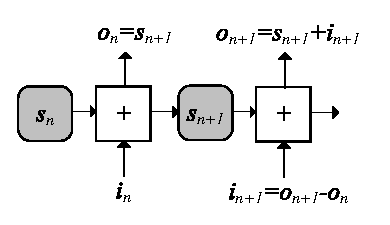
\includegraphics[width=0.3\textwidth]{mealy_add}
\end{center}
\caption{The circuit that breaks the causal relation}
  \label{mealy_add}
\end{figure}

\begin{equation}
\begin{array}{c}
s_{n+1}=i_n+s_n\\
o_{n}=i_n+s_n
\end{array}
\end{equation}

\textbf{Intuitively,
this circuit adds its input to its current state,
and puts the result to its output and next state.
So,
to recover the input letter $i_{n+1}$,
the output letter $o_n$ must be subtracted from $o_{n+1}$.
In this case,
$l$ is 1,
and $d$ is 0.
This explains why $l$ can be larger than $d$.
}

%\subsection{Craig Interpolation}\label{subsec_craig}



%\hfill mds
%
%\hfill January 11, 2007

%\subsection{Subsection Heading Here}
%Subsection text here.

% needed in second column of first page if using \IEEEpubid
%\IEEEpubidadjcol

%\subsubsection{Subsubsection Heading Here}
%Subsubsection text here.


% An example of a floating figure using the graphicx package.
% Note that \label must occur AFTER (or within) \caption.
% For figures, \caption should occur after the \includegraphics.
% Note that IEEEtran v1.7 and later has special internal code that
% is designed to preserve the operation of \label within \caption
% even when the captionsoff option is in effect. However, because
% of issues like this, it may be the safest practice to put all your
% \label just after \caption rather than within \caption{}.
%
% Reminder: the "draftcls" or "draftclsnofoot", not "draft", class
% option should be used if it is desired that the figures are to be
% displayed while in draft mode.
%
%\begin{figure}[!t]
%\centering
%\includegraphics[width=2.5in]{myfigure}
% where an .eps filename suffix will be assumed under latex,
% and a .pdf suffix will be assumed for pdflatex; or what has been declared
% via \DeclareGraphicsExtensions.
%\caption{Simulation Results}
%\label{fig_sim}
%\end{figure}

% Note that IEEE typically puts floats only at the top, even when this
% results in a large percentage of a column being occupied by floats.
% However, the Computer Society has been known to put floats at the bottom.


% An example of a double column floating figure using two subfigures.
% (The subfig.sty package must be loaded for this to work.)
% The subfigure \label commands are set within each subfloat command, the
% \label for the overall figure must come after \caption.
% \hfil must be used as a separator to get equal spacing.
% The subfigure.sty package works much the same way, except \subfigure is
% used instead of \subfloat.
%
%\begin{figure*}[!t]
%\centerline{\subfloat[Case I]\includegraphics[width=2.5in]{subfigcase1}%
%\label{fig_first_case}}
%\hfil
%\subfloat[Case II]{\includegraphics[width=2.5in]{subfigcase2}%
%\label{fig_second_case}}}
%\caption{Simulation results}
%\label{fig_sim}
%\end{figure*}
%
% Note that often IEEE papers with subfigures do not employ subfigure
% captions (using the optional argument to \subfloat), but instead will
% reference/describe all of them (a), (b), etc., within the main caption.


% An example of a floating table. Note that, for IEEE style tables, the
% \caption command should come BEFORE the table. Table text will default to
% \footnotesize as IEEE normally uses this smaller font for tables.
% The \label must come after \caption as always.
%
%\begin{table}[!t]
%% increase table row spacing, adjust to taste
%\renewcommand{\arraystretch}{1.3}
% if using array.sty, it might be a good idea to tweak the value of
% \extrarowheight as needed to properly center the text within the cells
%\caption{An Example of a Table}
%\label{table_example}
%\centering
%% Some packages, such as MDW tools, offer better commands for making tables
%% than the plain LaTeX2e tabular which is used here.
%\begin{tabular}{|c||c|}
%\hline
%One & Two\\
%\hline
%Three & Four\\
%\hline
%\end{tabular}
%\end{table}


% Note that IEEE does not put floats in the very first column - or typically
% anywhere on the first page for that matter. Also, in-text middle ("here")
% positioning is not used. Most IEEE journals use top floats exclusively.
% However, Computer Society journals sometimes do use bottom floats - bear
% this in mind when choosing appropriate optional arguments for the
% figure/table environments.
% Note that, LaTeX2e, unlike IEEE journals, places footnotes above bottom
% floats. This can be corrected via the \fnbelowfloat command of the
% stfloats package.

\section{A Halting Algorithm to Determine the Existence of the Decoder}\label{sec_exist}
\subsection{Determining the Non-existence of the Decoder}\label{subsec_deterNo}

$PC$ in Definition \ref{def_pcc} only defines how to determine the existence of the decoder $E^{-1}$.
But how to determine the non-existence of $E^{-1}$ is left undefined.
So the key to a halting algorithm is to find out a necessary and sufficient condition for the non-existence of $E^{-1}$.

According to Definition \ref{def_pcc} and Figure \ref{t1},
$E^{-1}$ exists if there is a parameter value tuple $<p,d,l>$,
such that $E\vDash PC(p,d,l)$ holds.
So,
intuitively,
$E^{-1}$ does not exist if for every parameter value tuple $<p,d,l>$,
another tuple $<p',d',l'>$ with $p'>p$,$l'>l$ and $d'>d$ can always be found,
such that $E\vDash PC(p',d',l')$ does not hold.

This case can be detected by the SAT instance in Figure \ref{fig_double_loop},
which is similar to Figure \ref{t1},
except that three new constraints are inserted to detect loops in state sequences $s_{n-p}^{n+d-l}$,$s_{n+d-l+1}^n$ and $s_{n+1}^{n+d}$.
\textbf{If this SAT instance is satisfiable for the parameter value $<p,d,l>$,
these three loops can be expanded in the following way:
Assume that the length of loops in $s_{n-p}^{n+d-l}$,$s_{n+d-l+1}^n$ and $s_{n+1}^{n+d}$ are $l_1$, $l_2$ and $l_3$ respectively,
and that these loops are expanded for $q$ times.
Then,
the SAT instance generated from this expanding is shown in Figure \ref{fig_double_loop_unfold}.
This expanded SAT instance corresponds to $F_{LN}(p",d",l")$,
where:}

\begin{figure}[t]
\begin{center}
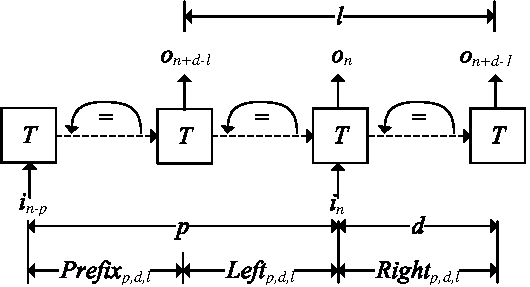
\includegraphics[width=0.45\textwidth]{doubleloop}
\end{center}
\caption{The loop-like non-complementary condition}
  \label{fig_double_loop}
\end{figure}


\begin{figure}[b]
\begin{center}
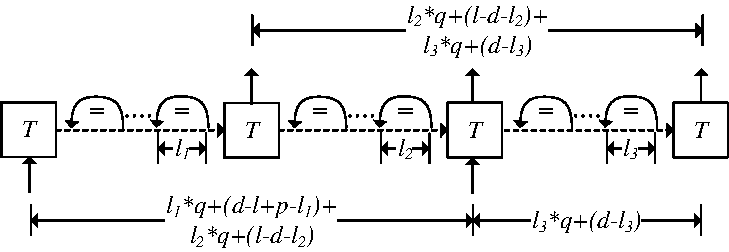
\includegraphics[width=0.45\textwidth]{doubleloop_unfold}
\end{center}
\caption{The loop-like non-complementary condition expanded for $q$ times}
  \label{fig_double_loop_unfold}
\end{figure}

\begin{equation}
\begin{array}{ccc}
p"&=&l_1*q+(d-l+p-l_1)+l_2*q+(l-d-l_2) \\
d"&=&l_3*q+(d-l_3) \\
l"&=&l_2*q+(l-d-l_2)+l_3*q+(d-l_3)
\end{array}
\end{equation}

\textbf{It is obvious that for every particular $<p,d,l>$ and $<p',d',l'>$,
there always exists a $q$,
such that $s_{n-p"}^{n+d"-l"}$,$s_{n+d"-l"+1}^n$ and $s_{n+1}^{n+d"}$ resulted from this expanding
are not shorter than $s_{n-p'}^{n+d'-l'}$,$s_{n+d'-l'+1}^n$ and $s_{n+1}^{n+d'}$ respectively.
The satisfiability of this expanded instance will be proved in Lemma \ref{lemma_unfold_longer} in next subsection.
This means for every particular $<p',d',l'>$,
we can always find another $<p",d",l">$,
such that $E\vDash PC(p",d",l")$ does not hold.
So the decoder does not exist.}



According to the 2nd and 3rd lines of Equation (\ref{uniqt1}),
there are actually two state sequences,
so these loops must be detected in both of them,
i.e.,
on the productive machine $M^2$ defined below:

\begin{definition11}%\addtolength{\itemsep}{-0.5\baselineskip}
%{\setlength{\baselineskip}{0.5\baselineskip}
\textbf{Productive machine :}
For Mealy machine $M=(S,s_0,I,O,T)$,
its Productive machine is $M^2=(S^2,s_0^2,I^2,O^2,T^2)$,
where
\begin{enumerate}
  \item $S^2=S\times S$
  \item $s_0^2=s_0\times s_0$
  \item $I^2=I\times I$
  \item $O^2=O\times O$
  \item $T^2$ is defined as $(<s_{m+1},s'_{m+1}>,<o_m,o'_m>)=T^2(<s_m,s'_m>,<i_m,i'_m>)$ with $(s_{m+1},o_m)=T(s_m,i_m)$ and $(s'_{m+1},o'_m)=T(s'_m,i'_m)$.
\end{enumerate}
\end{definition11}

Thus,
the loop-like non-complementary condition is formally defined below to determine the non-existence of $E^{-1}$:

\begin{definition11}\label{def_lnc}%\addtolength{\itemsep}{-0.5\baselineskip}
%{\setlength{\baselineskip}{0.5\baselineskip}
\textbf{Loop-like Non-complementary Condition ($\boldsymbol{LN}$) :}
For encoder $E$ and its Mealy machine $M=(S,s_0,I,O,T)$,
assume its productive machine is $M^2=(S^2,s_0^2,I^2,O^2,T^2)$,
then $E\vDash LN(p,d,l)$ holds if
$i_n$ can not be uniquely determined by $o_{n+d-l}^{n+d-1}$ in the state sequence $s_{n-p}^{n+d-1}$,
and there are loops in $(s^2)_{n-p}^{n+d-l}$,$(s^2)_{n+d-l+1}^n$ and $(s^2)_{n+1}^{n+d}$.
This equals the satisfiability of $F_{LN}(p,d,l)$ in Equation (\ref{uniqln}).
$E\vDash LN$ is further defined as $\exists p,d,l:E\vDash LN(p,d,l)$.
\end{definition11}


\begin{equation}\label{uniqln}
\begin{split}
&F_{LN}(p,d,l)\overset{def}{=}\\
&\left\{
\begin{array}{cc}
&\bigwedge_{m=n-p}^{n+d-1}
\{
(s_{m+1},o_m)\equiv T(s_m,i_m)
\}
\\
\wedge&\bigwedge_{m=n-p}^{n+d-1}
\{
(s'_{m+1},o'_m)\equiv T(s'_m,i'_m)
\}
\\
\wedge&\bigwedge_{m=n+d-l}^{n+d-1}o_m\equiv o'_m \\
\wedge& i_n\ne i'_n \\
\wedge&\bigvee_{x=n-p}^{n+d-l-1}\bigvee_{y=x+1}^{n+d-l} \{s_x\equiv s_y\wedge s'_x\equiv s'_y\} \\
\wedge&\bigvee_{x=n+d-l+1}^{n-1}\bigvee_{y=x+1}^{n} \{s_x\equiv s_y\wedge s'_x\equiv s'_y\} \\
\wedge&\bigvee_{x=n+1}^{n+d-1}\bigvee_{y=x+1}^{n+d} \{s_x\equiv s_y\wedge s'_x\equiv s'_y\}
\end{array}
\right\}
\end{split}
\end{equation}



By comparing Equations (\ref{uniqt1}) and (\ref{uniqln}),
it is obvious that their only difference is the last three newly inserted lines in (\ref{uniqln}),
which will be used to detect loops in the following three state sequences:
\begin{equation}
\begin{array}{ccc}
Prefix_{p,d,l}&=&(s^2)_{n-p}^{n+d-l} \\
Left_{p,d,l}&=&(s^2)_{n+d-l+1}^n \\
Right_{p,d,l}&=&(s^2)_{n+1}^{n+d}
\end{array}
\end{equation}


The correctness of this approach will be proved in the next subsection.




\subsection{Proving Correctness}

Before proving correctness of this approach,
some lemmas are needed.
\begin{figure}[b]
\centering
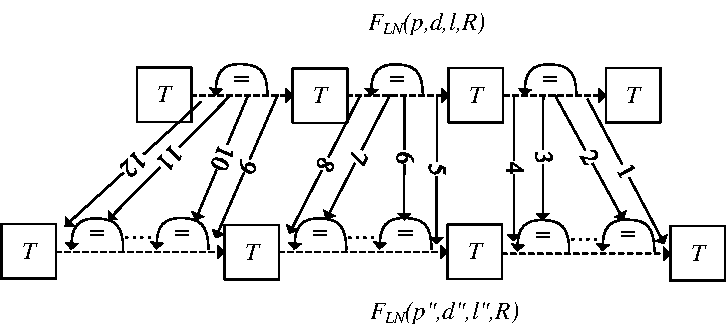
\includegraphics[width=0.45\textwidth]{doubleloop_unfold_cmp}
\caption{Correspondence between $F_{LN}(p,d,l)$ and $F_{LN}(p",d",l")$}
\label{doubleloop_unfold_cmp}
\end{figure}


\begin{lemma}[]\label{lemma_unfold_longer}
For $F_{LN}(p",d",l")$ in Figure \ref{fig_double_loop_unfold},
$E\vDash LN(p,d,l)$ implies $E\vDash LN(p",d",l")$.
\end{lemma}
\begin{proof}
The formula $F_{LN}(p",d",l")$ is:

\begin{equation}\label{equ_correspondance}
\begin{split}
&F_{LN}(p",d",l")\stackrel{def}{=}\\
&\left\{
\begin{array}{cc}
&\bigwedge_{m=n-p"}^{n+d"-1}
\{
(s_{m+1},o_m)\equiv T(s_m,i_m)
\}
\\
\wedge&\bigwedge_{m=n-p"}^{n+d"-1}
\{
(s'_{m+1},o'_m)\equiv T(s'_m,i'_m)
\}
\\
\wedge&\bigwedge_{m=n+d"-l"}^{n+d"-1}o_m\equiv o'_m \\
\wedge& i_n\ne i'_n \\
\wedge& \bigvee_{x=n-p"}^{n+d"-l"-1}\bigvee_{y=x+1}^{n+d"-l"} \{s_x\equiv s_y\wedge s'_x\equiv s'_y\} \\
\wedge& \bigvee_{x=n+d"-l"+1}^{n-1}\bigvee_{y=x+1}^{n} \{s_x\equiv s_y\wedge s'_x\equiv s'_y\} \\
\wedge& \bigvee_{x=n+1}^{n+d"-1}\bigvee_{y=x+1}^{n+d"} \{s_x\equiv s_y\wedge s'_x\equiv s'_y\}
\end{array}
\right\}
\end{split}
\end{equation}

$E\vDash LN(p,d,l)$ means that $F_{LN}(p,d,l)$ is satisfied.
Assume its satisfying assignment is $A$.
%We need to prove that $F_{LN}(p",d",l")$ is also satisfied with $A$.
The directed arcs numbered from 1 to 12 in Figure \ref{doubleloop_unfold_cmp}
show the correspondence between $F_{LN}(p,d,l)$ and $F_{LN}(p",d",l")$.

The arcs 2 and 3 mean applying the satisfying assignment of the loop in $Right_{p,d,l}$
to the expanded loops in $Right_{p",d",l"}$.
The arcs 1 and 4 mean applying the satisfying assignments of the two state sequences that is not in the loop,
to $Right_{p",d",l"}$.
With the arcs 1,2,3 and 4,
the state sequence $Right_{p",d",l"}$ is satisfied.

Similarly,
the state sequences $Prefix_{p",d",l"}$ and $Left_{p",d",l"}$ can also be satisfied with $A$.
Thus the 2nd line of Equation (\ref{equ_correspondance}) is satisfied with the assignment $A$.

Similarly,
the 3rd to 5th lines of Equation (\ref{equ_correspondance}) are also satisfied with the assignment $A$.

At the same time,
there are $q$ loops in $Prefix_{p",d",l"}$, $Left_{p",d",l"}$ and $Right_{p",d",l"}$,
which will make the last three lines in Equation (\ref{equ_correspondance}) satisfied.

Thus,the satisfying assignment $A$ of $F_{LN}(p,d,l)$ can also make $F_{LN}(p",d",l")$ satisfied.
This concludes the proof.
\end{proof}

\begin{lemma}[]\label{lemma_pc_long}
For two tuples $<p,d,l>$ and $<p',d',l'>$,
if $Prefix_{p',d',l'}$,$Left_{p',d',l'}$ and $Right_{p',d',l'}$ are \textbf{not shorter} than $Prefix_{p,d,l}$,$Left_{p,d,l}$ and $Right_{p,d,l}$ respectively,
then $E\vDash PC(p,d,l)\to E\vDash PC(p',d',l')$.
\end{lemma}
\begin{proof}
It is obvious that $F_{PC}(p,d,l)$ is a sub-formula of $F_{PC}(p',d',l')$,
so the unsatisfiability of the former one implies the unsatisfiability of the latter one.
Thus,
$E\vDash PC(p,d,l)\to E\vDash PC(p',d',l')$ holds.
\end{proof}

The following two theorems will prove that $E\vDash LN\leftrightarrow \neg \{E\vDash PC\}$.



\begin{theorem}[]\label{thm_pc_nln}
$E\vDash LN\to \neg \{E\vDash PC\}$
\end{theorem}
\begin{proof}
This can be proved by contradiction.
Assume that $E\vDash LN$ and $E\vDash PC$ both hold.
This means there exist $<p,d,l>$ and $<p',d',l'>$,
such that $E\vDash PC(p,d,l)$ and $E\vDash LN(p',d',l')$.

On the one hand,
$E\vDash LN(p',d',l')$ implies that there are loops in the state sequences $Prefix_{p',d',l'}$,$Left_{p',d',l'}$ and $Right_{p',d',l'}$.
By expanding these loops,
another tuple $<p",d",l">$ can be found,
so that :
\begin{enumerate}
\item $Prefix_{p",d",l"}$,$Left_{p",d",l"}$ and $Right_{p",d",l"}$ are not shorter than $Prefix_{p,d,l}$,$Left_{p,d,l}$ and $Right_{p,d,l}$ respectively;
\item According to Lemma \ref{lemma_unfold_longer},
$F_{LN}(p",d",l")$ is satisfiable.
\end{enumerate}

$F_{PC}(p",d",l")$ is a sub-formula of $F_{LN}(p",d",l")$,
so $F_{PC}(p",d",l")$ is also satisfiable,
which means that $E\vDash PC(p",d",l")$ does not hold.

On the other hand,
according to Lemma \ref{lemma_pc_long},
$E\vDash PC(p",d",l")$ holds.

This contradiction concludes the proof.
\end{proof}

\begin{theorem}[]\label{thm_nln_pc}
$E\vDash LN\gets \neg \{E\vDash PC\}$
\end{theorem}
\begin{proof}
Let's prove it by contradiction.
Assume that neither $E\vDash LN$ nor $E\vDash PC$ holds.
Then for every $<p,d,l>$ and $<p',d',l'>$,
$F_{PC}(p,d,l)$ is satisfiable,
while $F_{LN}(p',d',l')$ is unsatisfiable.

Thus,
assume the $uirrd(M^2)$ is the uninitialized state variables recurrence diameter of $E$'s productive machine.
Let's define $<p,d,l>$ as:
\begin{equation}
\begin{array}{c}
p=uirrd(M^2)*2+2 \\
d=uirrd(M^2)+1 \\
l=uirrd(M^2)*2+2
\end{array}
\end{equation}

With this definition,
it is obvious that $Prefix_{p,d,l}$,$Left_{p,d,l}$ and $Right_{p,d,l}$ are both longer than $uirrd(M^2)$.
This means that there are loops in all these three state sequences,
which will make $F_{LN}(p,d,l)$ satisfiable.
This contradicts with the fact that $F_{LN}(p',d',l')$ is unsatisfiable for every $<p',d',l'>$.

This contradiction concludes the proof.
\end{proof}

Theorems \ref{thm_pc_nln} and \ref{thm_nln_pc} illustrate that,
a halting algorithm can be implemented by
enumerating all combinations of $<p,d,l>$ from small to large,
and checking $E\vDash PC(p,d,l)$ and $E\vDash LN(p,d,l)$ in every iteration.
This process will eventually terminate with one and only one answer between $E\vDash PC$ and $E\vDash LN$.
The implementation of this algorithm will be presented in the next subsection.

\subsection{Algorithm Implementation}\label{subsec_algoimp}

\begin{algorithm}
\caption{$check\_PCLN$}
\label{algo_pcln}
\begin{algorithmic}[1]
\FOR{$x=1 \to \infty$}
    \STATE{$p=2x$}
    \STATE{$d=x$}
    \STATE{$l=2x$}
      \IF{$F_{PC}(p,d,l)$ is unsatisfiable}
        \PRINT \texttt{"$E^{-1}$ exists with $<p,d,l>$"}\label{lab_pc}
        \STATE \textbf{halt};
      \ELSIF{$F_{LN}(p,d,l)$ is satisfiable}
        \PRINT \texttt{"$E^{-1}$ does not exist"}\label{lab_ln}
        \STATE \textbf{halt};
      \ENDIF
\ENDFOR
\end{algorithmic}
\end{algorithm}

\begin{figure}[b]
\begin{center}
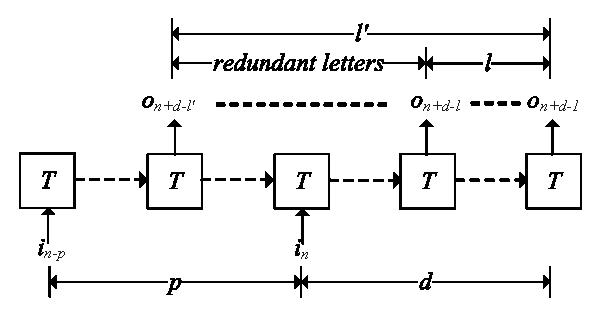
\includegraphics[width=0.45\textwidth]{rmred}
\end{center}
\caption{The Redundant Output Letters}
  \label{fig_rmred}
\end{figure}

\textbf{Instead of enumerating all combinations of parameter value $p$, $d$ and $l$ like \cite{ShengYuShen:iccad09,ShengYuShen:tcad},
Line 2,3 and 4 of Algorithm \ref{algo_pcln} ensure that the lengths of $Prefix_{p,d,l}$,$Left_{p,d,l}$ and $Right_{p,d,l}$ are all set to $x$, 
which is enumerated at Line 1.
In this way,
the run time overhead is further reduced because many redundant combinations do not need to be tested any more.}



According to Theorems \ref{thm_pc_nln} and \ref{thm_nln_pc},
Algorithm \ref{algo_pcln} will eventually terminate at line \ref{lab_pc} or \ref{lab_ln}.

\section{Removing Redundant Output Letters}\label{sec_rmred}
\begin{algorithm}
\caption{$RemoveRedundancy(p,d,l)$}
\label{algo_remove}
\begin{algorithmic}[1]
\FOR{$p'=p \to 0$}
  \IF{$F_{PC}(p'-1,d,l)$ is satisfiable}
    \STATE break
  \ENDIF
\ENDFOR
\FOR{$d'=d \to 0$}
  \IF{$F_{PC}(p',d'-1,l)$ is satisfiable}
    \STATE break
  \ENDIF
\ENDFOR
\FOR{$l'=1 \to l-(d-d')$}
  \IF{$F_{PC}(p',d',l')$ is unsatisfiable}
    \STATE break
  \ENDIF
\ENDFOR
\PRINT \texttt{"final result is $<p',d',l'>$"}
\end{algorithmic}
\end{algorithm}

Although Algorithm \ref{algo_pcln} is sufficient to determine the existence of $E^{-1}$,
the parameter values found by line \ref{lab_pc} of Algorithm \ref{algo_pcln} contain some redundancy,
which will cause unnecessarily large overheads on the circuit area and the run time of characterizing.

For example,
as shown in Figure \ref{fig_rmred},
assume that $l$ is the smallest parameter value that leads to $E\vDash PC(p,d,l)$,
and $l<d$,
which means that $i_n$ is uniquely determined by some output letters $o_k$ with $k>n$.
Further assume that line \ref{lab_pc} of Algorithm \ref{algo_pcln} prove $E\vDash PC(p,d,l')$.
It is obvious that $l'>d$,
which makes $i_n$ depend on some redundant $o_k$ with $k\le n$.
So $o_{n+d-l'}^{n+d-l-1}$ is the sequence of redundant output letters,
which should be removed to prevent them from being instantiated as latches in circuit $E^{-1}$.
At the same time,
also according to Figure \ref{fig_rmred},
larger $p$ and $d$ lead to larger SAT instances for the characterization algorithm in the 2nd step of complementary synthesis.

So,
Algorithm \ref{algo_remove} is used to minimize $<p,d,l>$ before passing it to the characterization algorithm:




\section{Experimental Results}\label{sec_exp}
This algorithm has been implemented with the OCaml language.
The generated SAT instances are solved with Zchaff SAT solver\cite{CHAFF}.
All experiments are run on a PC with a 2.4GHz Intel Core 2 Q6600 processor, 8GB memory and CentOS 5.2 linux.
All these experimental results and programs can be downloaded from \url{http://www.ssypub.org}.
%All related programs and data files can be downloaded from \url{http://www.ssypub.org}.
\subsection{Benchmarks}
\begin{table}[t]
\centering
\caption{Information of Benchmarks}
\begin{tabular}{|c|c|c|c|c|c|}
\hline
&XGXS&XFI&scrambler&PCI-E&T2 et-\\
&&&&&hernet\\\hline
Line number&&&&&\\
of verilog&214&466&24&1139&1073\\
source code&&&&&\\\hline
\#regs&15&135&58&22&48\\\hline
Data path&8&64&66&10&10\\
width&&&&&\\ \hline
\end{tabular}\label{tab_info}
\end{table}


Table \ref{tab_info} shows the information of the following benchmarks.
\begin{enumerate}

\item A XGXS encoder that is compliant to clause 48 of IEEE-802.3ae 2002 standard \cite{IEEE80232002}.

\item A XFI encoder that is compliant to clause 49 of the same IEEE standard.

\item A 66-bit scrambler that is used to ensure
that a data sequence has sufficiently many 0-1 transitions
, so that it can run through a high-speed
noisy serial transmission channel.

\item A PCI-E physical coding module \cite{PCIESPEC}.

\item The Ethernet module of Sun's OpenSparc T2 processor.
\end{enumerate}

\subsection{Determining the existence of the decoder for Properly Designed Encoders}\label{subsec_prop}
\begin{table}[b]
\centering
\caption{Experimental Results on Properly Designed Encoders}
\begin{tabular}{|c|c|c|c|c|c|c|}
\hline
&                                        &XGXS     &XFI       &scra-     &PCI-E    &T2 et-\\
&                                        &         &          &mbler     &        &hernet\\ \hline
&Time to ch-                           &&&&&\\
\cite{ShengYuShen:fmcad10}&eck $PC$(sec)     &1.06     &70.52     &5.74      &2.40    &66.37\\\cline{2-7}
&$d,p,l$                                 &1,1,1    &0,3,2     &0,2,2     &2,1,1   &4,1,1         \\ \hline\hline
This&Time to ch-                         &&&&&\\
paper&eck $PC$(sec)                           &0.29     &17.86     &2.67      &0.47    &29.64\\\cline{2-7}
&$d,p,l$                                 &1,2,1    &0,3,2     &0,2,2     &2,2,1   &4,4,1          \\ \hline
\end{tabular}\label{tab_prodes}
\end{table}

The 2nd and 4th rows of Table \ref{tab_prodes} compare the run time of checking $E\vDash PC$ between \cite{ShengYuShen:fmcad10} and this paper.
It is obvious that this paper's approach is much faster than that of \cite{ShengYuShen:fmcad10}.

The 3rd and 5th rows compare the discovered parameter values,
and some minor differences are found on parameter value $p$.
This is caused by the different orders in checking various parameter combinations.

\subsection{Comparing Decoder Area}\label{subsec_area}

Table \ref{tab_cmparea} compares the circuit area of the decoders built manually,
and the decoders built by this paper's algorithm.
These decoders are synthesized with LSI10K technology library from Synopsys DesignCompiler.

\begin{table}[t]
\centering
\caption{Comparing Decoder Area}
\begin{tabular}{|c|c|c|c|c|c|}
\hline
                   &XGXS      &XFI       &scrambler    &PCI-E  &T2 et-\\
&&&&&hernet\\ \hline
The decoders       &921       &6002      &1629         &852   &1446          \\
built manually           &&&&&\\ \hline
The decoders built by      &700       &12754     &1455         &455   &552          \\
this paper's algorithm   &&&&&\\ \hline
\end{tabular}\label{tab_cmparea}
\end{table}

\textbf{From Table \ref{tab_cmparea},
it is obvious that,
except for the most complex XFI, synthesis results of this paper's algorithm
are more compact than those decoders built manually. However,
this comparison is unfair because those decoders built manually
include additional functionality, 
such as testing logic.}

\textbf{On the other hand,
for XFI,
the circuit area of this paper's algorithm is about 2 times larger.
This means the circuit area must be improved in the future work.}


\subsection{Comparing Decoder Timing}\label{subsec_timing}

\begin{table}[b]
\centering
\caption{Comparing Critical Path Latencies in nanosecond}
\begin{tabular}{|c|c|c|c|c|c|}
\hline
                   &XGXS        &XFI       &scrambler    &PCI-E   &T2 et-\\
&&&&&hernet\\ \hline
The decoders       &12.33       &46.65     &6.54         &19.03  &23.36          \\
built manually           &&&&&\\ \hline
The decoders built by      &11.96       &28.13     &6.54         &9.09   &12.69          \\
this paper's algorithm   &&&&&\\ \hline
\end{tabular}\label{tab_cmptiming}
\end{table}

\begin{table}[t]
\centering
\caption{Comparing Run time of Improperly Designed Encoders}
\begin{tabular}{|c|c|c|c|c|c|c|}
\hline
                                        &XGXS     &XFI       &scra-     &PCI-E    &T2 et-\\
                                        &         &          &mbler     &        &hernet\\ \hline
The algorithm      &&&&&\\
of \cite{ShengYuShen:fmcad10}(sec)     &0.98     &35.08     &2.54      &1.36    &17.39\\\hline
This paper's                         &&&&&\\
algorithm(sec)                           &0.16     &7.59     &1.17      &0.33    &2.19\\\hline
\end{tabular}\label{tab_impdes}
\end{table}


\textbf{Table \ref{tab_cmptiming} compares the critical path latencies of the decoders built manually
and the decoders built by this paper's algorithm.
Their synthesis settings are the same as Subsection \ref{subsec_area}.
For all those circuits,
the critical path latencies of the decoders built by this paper's algorithm are all better.}

%The only exception is XFI,
%the latency of the decoder built by our algorithm is significantly larger than that of hand-written decoder.
%
%One interesting issue that is not shown in Table \ref{tab_cmptiming} is,
%all these critical paths start from registers, and end at output ports.



\subsection{Determining the non-existence of the decoder for Improperly Designed Encoders}\label{subsec_improp}
To further show the usefulness of this paper's algorithm,
some improperly designed encoders without corresponding decoders are needed.
These improperly designed encoders are obtained by modifying each benchmark's output statements,
so that they can explicitly output the same letter for two different input letters.
In this way,
input letter $i_n$ can never be uniquely determined by $E$'s output sequence.

The 2nd row of Table \ref{tab_impdes} shows the run time of \cite{ShengYuShen:fmcad10} on checking these improperly designed encoders,
while the 3rd row shows the run time of this paper's algorithm.
These results indicate that this paper's algorithm always terminate correctly,
and is much faster than \cite{ShengYuShen:fmcad10}.


\section{Related Works}\label{sec_relwork}
%\subsection{Complementary Synthesis}
%%Complementary synthesis is an emerging new research topic,
%%there are only two papers that discuss this problem.
%
%The concept of complementary synthesis was first proposed by us\cite{ShengYuShen:iccad09} in ICCAD 2009.
%Its major shortcomings are that it is incomplete,
%and its run-time overhead of building decoder is too large.
%
%The incomplete problem has been addressed by \cite{ShengYuShen:fmcad10}, while \cite{ShengYuShen:tcad} addresses the second shortcoming by simplifying the SAT instance with unsatisfiable core extraction before building decoders.

\subsection{Complementary Synthesis}\label{subsec_compsyn_relat}
\textbf{The concept of complementary synthesis was first proposed by us\cite{ShengYuShen:iccad09} in ICCAD 2009.
Its major shortcomings are that it is not halting,
and its run-time overhead of building complementary circuit is too large.}

\textbf{The halting problem was handled by building a set of over-approximations that are similar to onion rings \cite{ShengYuShen:fmcad10},
while the run-time overhead problem was addressed by simplifying the SAT instance with unsatisfiable core extraction\cite{ShengYuShen:tcad}.}

\subsection{Program Inverse}\label{subsec_proinv}
\textbf{According to Gulwani\cite{dim_syn},
program inverse is the problem that derives a program $P^{-1}$
that negates the computation of a given program $P$.
So the definition of program inverse is very similar to complementary synthesis.}

\textbf{The initial work on deriving program inverse used proof-based approaches\cite{prog_inv},
but it could only handle very small programs and very simple syntax structures.}

\textbf{Gl\"{u}ck et.al \cite{mtd_autoProginv} inversed the first-order functional programs
by eliminating nondeterminism with LR-based parsing methods.
The requirement that the program to be inversed should be expressed in a functional language make it impossible to be applied to complementary synthesis.}

\textbf{Srivastava et.al \cite{prog_inv_rev} assumed that an inverse program was typically related to the original program,
so the space of possible inverses can be inferred by automatically
mining the original program for expressions, predicates, and control flow.
This algorithm inductively rules out invalid paths that can't fulfill the requirement of inversion,
to narrow down the space of candidate programs until only the valid ones remain.
So it can only guarantee the existence of a solution,
but not the correctness of this solution if its assumptions do not hold.}



\subsection{The Completeness of Bounded Model Checking}\label{subsec_bmc_relate}
Bounded model checking(BMC) \cite{bmc_tacas99} is a model checking technology that considers only the paths of limited length.
So it is an incomplete algorithm.
Many researchers try to find out complete approaches for BMC.

One line of research\cite{bmc_tacas99,RecDiam} tried to find out a bound $b$,
which can guarantee the correctness of a specification,
if the specification is correct on all paths that are shorter than $b$.
\textbf{Line 8 of Algorithm \ref{algo_pcln} finds out the value of $p$,$d$ and $l$ that can prove the non-existence of the decoder.
This is similar to these related researches.}

The other line of research\cite{kind_tacas99} tried to find out a pattern for induction,
such that the correctness of a specification within any bound $b$ implies the correctness on bound $b+1$.
\textbf{Our algorithm proves the non-existence of the decoder by expanding loops.
This is similar to finding induction pattern in this related research.}

% \textbf{This paper achieves completeness without following these two approaches.
% Instead,
% it defines two complement uniqueness conditions,
% $LP$ and $LL$,
% and find out proper algorithms to check them.}

%\subsection{Temporal Logic Synthesis}
%%Automatically synthesis of program from logic specification is first identified as Church's problem in 1962\cite{LOGARTHAUTO}.
%%Some early researches \cite{SLVSQFSS,AUTOINF} solve this problem by reducing it to checking emptiness of tree automata.
%
%The temporal logic synthesis was first addressed by Clarke et.al\cite{DSGSYNTMPLG} and Manna et.al \cite{SYNTMPLGSPC}.
%But Pnueli et.al \cite{SYNRCTVMD} pointed out that the complexity of LTL synthesis is double exponent.
%%This high complexity drives researchers turning their focus to find smaller but still useful subset of temporal logic,
%%such that synthesis problem can be solved with lower complexity.
%
%One line of research \cite{CNTLSYNTMDAUTO,DTMGENGMELTL,SYNRCTVDES} focuses on the so-called generalized reactive formulas of the form:
%$(\square \lozenge p_1 \wedge \cdots \square \lozenge p_m) \to (\square \lozenge q_1 \wedge \cdots \square \lozenge q_n)$.
%Complexity of solving synthesis problem for such formula is $O(N^3)$.
%
%The other line of research focuses on finding efficient algorithm \cite{SYNCNTLBNDRPN}
%for expensive safra determination algorithm \cite{CMPLXAUTO} on an useful formula subset,
%or just avoiding it\cite{NEWALGSTRGSYN}.
%
%%Yet another approach is antichain\cite{ANTICHAIN},
%%which reduces the expensive state set computation to computation on maximal and minimal elements of lattice.
%
%Based on these research works,
%some tools\cite{ANZU} that can handle small temporal formulas have been developed.
%
%All these works assume a hostile environment,
%which seems too restrictive for many applications.
%So Fisman et.al \cite{rationalsyn_tacas10}, Chatterjee et.al \cite{assguasyn_tacas07} and Ummels et.al \cite{ralgame_istta06} proposed rational synthesis algorithm,
%which assumes that each agents act to achieve their own goals instead of failing each other.


\subsection{Protocol Converter Synthesis}
The protocol converter synthesis is the problem that automatically generates a translator between two different communication protocols.
\textbf{This is related to our works because both of us focus on synthesizing communication circuits.}

Avnit et.al \cite{converter_date08,converter_todeas09} first defined a general model for describing the different protocols.
Then it provided an algorithm to decide
whether there are some functionality of a protocol that can't be translated into another.
Finally,
it synthesized the translator by computing a greatest fixed point for the update function of the buffer's control states.
Avnit et.al\cite{converter_date09} improved the algorithm mentioned above with a more efficient design space exploration algorithm.

%This paper address the first shortcoming.

\section{Conclusions}\label{sec_conclude}

This paper proposes a faster and more straightforward halting algorithm that checks whether a particular encoder has its corresponding decoder.
The theoretical analysis shows that this paper's approach always distinguishes correct encoders from their incorrect variants and halts properly.
Experimental results show that this paper's approach is much faster than that of \cite{ShengYuShen:fmcad10}.


%At the same time,
%we propose to characterize the Boolean function of $E^{-1}$ with interpolation.
%Experimental results show that our approach can be one order of magnitude faster than our previous work\cite{ShengYuShen:tcad}.
%
%One future work is to develop a debugging method to find out why $E^{-1}$ does not exist.
%For the failure caused by loop-like path,
%we plan to develop a debugging mechanism based on our previous work on loop-like counterexample minimization \cite{ShengYuShen:charme05}.

\section*{Acknowledgment}
The authors would like to thank the editors and anonymous reviewers for their hard work.

This work was funded by projects 60603088 and 61070132 supported by National Natural Science Foundation of China.

% An example of a floating figure using the graphicx package.
% Note that \label must occur AFTER (or within) \caption.
% For figures, \caption should occur after the \includegraphics.
% Note that IEEEtran v1.7 and later has special internal code that
% is designed to preserve the operation of \label within \caption
% even when the captionsoff option is in effect. However, because
% of issues like this, it may be the safest practice to put all your
% \label just after \caption rather than within \caption{}.
%
% Reminder: the "draftcls" or "draftclsnofoot", not "draft", class
% option should be used if it is desired that the figures are to be
% displayed while in draft mode.
%
%\begin{figure}[!t]
%\centering
%\includegraphics[width=2.5in]{myfigure}
% where an .eps filename suffix will be assumed under latex,
% and a .pdf suffix will be assumed for pdflatex; or what has been declared
% via \DeclareGraphicsExtensions.
%\caption{Simulation Results}
%\label{fig_sim}
%\end{figure}

% Note that IEEE typically puts floats only at the top, even when this
% results in a large percentage of a column being occupied by floats.


% An example of a double column floating figure using two subfigures.
% (The subfig.sty package must be loaded for this to work.)
% The subfigure \label commands are set within each subfloat command, the
% \label for the overall figure must come after \caption.
% \hfil must be used as a separator to get equal spacing.
% The subfigure.sty package works much the same way, except \subfigure is
% used instead of \subfloat.
%
%\begin{figure*}[!t]
%\centerline{\subfloat[Case I]\includegraphics[width=2.5in]{subfigcase1}%
%\label{fig_first_case}}
%\hfil
%\subfloat[Case II]{\includegraphics[width=2.5in]{subfigcase2}%
%\label{fig_second_case}}}
%\caption{Simulation results}
%\label{fig_sim}
%\end{figure*}
%
% Note that often IEEE papers with subfigures do not employ subfigure
% captions (using the optional argument to \subfloat), but instead will
% reference/describe all of them (a), (b), etc., within the main caption.


% An example of a floating table. Note that, for IEEE style tables, the
% \caption command should come BEFORE the table. Table text will default to
% \footnotesize as IEEE normally uses this smaller font for tables.
% The \label must come after \caption as always.
%
%\begin{table}[!t]
%% increase table row spacing, adjust to taste
%\renewcommand{\arraystretch}{1.3}
% if using array.sty, it might be a good idea to tweak the value of
% \extrarowheight as needed to properly center the text within the cells
%\caption{An Example of a Table}
%\label{table_example}
%\centering
%% Some packages, such as MDW tools, offer better commands for making tables
%% than the plain LaTeX2e tabular which is used here.
%\begin{tabular}{|c||c|}
%\hline
%One & Two\\
%\hline
%Three & Four\\
%\hline
%\end{tabular}
%\end{table}


% Note that IEEE does not put floats in the very first column - or typically
% anywhere on the first page for that matter. Also, in-text middle ("here")
% positioning is not used. Most IEEE journals use top floats exclusively.
% Note that, LaTeX2e, unlike IEEE journals, places footnotes above bottom
% floats. This can be corrected via the \fnbelowfloat command of the
% stfloats package.



%\section{Conclusion}
%The conclusion goes here.





% if have a single appendix:
%\appendix[Proof of the Zonklar Equations]
% or
%\appendix  % for no appendix heading
% do not use \section anymore after \appendix, only \section*
% is possibly needed

% use appendices with more than one appendix
% then use \section to start each appendix
% you must declare a \section before using any
% \subsection or using \label (\appendices by itself
% starts a section numbered zero.)
%


%\appendices
%\section{Proof of the First Zonklar Equation}
%Appendix one text goes here.

% you can choose not to have a title for an appendix
% if you want by leaving the argument blank
%\section{}
%Appendix two text goes here.


% use section* for acknowledgement
%\section*{Acknowledgment}

%The authors would like to thank the anonymous reviewer's time and effort.

%This work is fund by Chinese National Science Foundation No.60603088.


% Can use something like this to put references on a page
% by themselves when using endfloat and the captionsoff option.
\ifCLASSOPTIONcaptionsoff
  \newpage
\fi



% trigger a \newpage just before the given reference
% number - used to balance the columns on the last page
% adjust value as needed - may need to be readjusted if
% the document is modified later
%\IEEEtriggeratref{8}
% The "triggered" command can be changed if desired:
%\IEEEtriggercmd{\enlargethispage{-5in}}

% references section

% can use a bibliography generated by BibTeX as a .bbl file
% BibTeX documentation can be easily obtained at:
% http://www.ctan.org/tex-archive/biblio/bibtex/contrib/doc/
% The IEEEtran BibTeX style support page is at:
% http://www.michaelshell.org/tex/ieeetran/bibtex/
%\bibliographystyle{IEEEtran}
% argument is your BibTeX string definitions and bibliography database(s)
%\bibliography{IEEEabrv,../bib/paper}
%
% <OR> manually copy in the resultant .bbl file
% set second argument of \begin to the number of references
% (used to reserve space for the reference number labels box)
\begin{thebibliography}{1}

\bibitem{ShengYuShen:iccad09}
S. Shen, J. Zhang, Y. Qin, and S. Li,
"Synthesizing complementary circuits automatically,"
in Proc. IEEE ICCAD, Nov. 2009, pp. 381-388.

\bibitem{ShengYuShen:tcad}
S. Shen, Y. Qin, K. Wang, L. Xiao, J. Zhang, and S. Li,
"Synthesizing Complementary Circuits Automatically,"
IEEE Trans. Comput.-Aided Design Integr. Circuits Syst.,
vol. 29, no. 8, pp. 1191-1202, Aug. 2010.


\bibitem{ShengYuShen:fmcad10}
S. Shen, Y. Qin, J. Zhang, and S. Li,
"A Halting Algorithm to Determine the Existence of Decoder,"
in Proc. IEEE FMCAD, Oct. 2010, pp. 91-100.

\bibitem{CHAFF}
M. W. Moskewicz, C. F. Madigan, Y. Zhao, L. Zhang, and S. Malik,
"Chaff: Engineering an efficient SAT solver," in Proc. IEEE Int. DAC,
Jun. 2001, pp. 530-535.


\bibitem{PCIESPEC}
"PCI Express Base Specification Revision 1.0". [Online]. Available:
  \url{http://www.pcisig.com}

\bibitem{IEEE80232002}
"IEEE Standard for Information technology Telecommunications and
  information exchange between systems Local and metropolitan area networks
  Specific requirements Part 3: Carrier Sense Multiple Access with Collision
  Detection (CSMA/CD) Access Method and Physical Layer Specifications
  Amendment: Media Access Control (MAC) Parameters, Physical Layers, and
  Management Parameters for 10 Gb/s Operation", IEEE Std. 802.3, 2002.

\bibitem{CoreGen}
Xilinx. (2008) Xilinx core generator system. [Online]. Available:
  \url{http://www.xilinx.com/tools/coregen.htm}


\bibitem{DesignWare}
Synopsys. (2008) Designware library. [Online]. Available:
  \url{http://www.synopsys.com/IP/DESIGNWARE/Pages/default.aspx}


\bibitem{grasp}
J. P. M. Silva and K. A. Sakallah,
"GRASP - a new search algorithm for satisfiability,"
in Proc. IEEE ICCAD, Nov. 1996, pp. 220-227.


\bibitem{BERKMIN}
E. Goldberg and Y. Novikov,
"BerkMin: A fast and robust Sat-solver,"
Discrete Applied Mathematics,
vol. 155, no. 12,
pp. 1549-1561, Dec. 2007.

\bibitem{EXTSAT}
N. E\'en and N. S\"orensson.,
"Extensible SAT-solver,"
in Proc. Int. Conf.
SAT, May 2003, pp. 502-518.

\bibitem{MEALY}
G. H. Mealy , "A method for synthesizing sequential circuits," Bell Syst.
Tech. J., vol. 34, pp. 1045-1079, Jan. 1955.


\bibitem{RecDiam}
D. Kroening and O. Strichman,
"Efficient Computation of Recurrence Diameters,"
in Proc. Int. Conf. VMCAI, Jan. 2003,
pp. 298-309.



\bibitem{TH1A}
"China Grabs Supercomputing Leadership Spot in Latest Ranking of World's Top 500 Supercomputers". [Online]. Available: \url{http://www.top500.org/lists/2010/11/press-release}.





\bibitem{bmc_tacas99}
E. M. Clarke, A. Biere, R. Raimi, and Y. Zhu,
"Bounded Model Checking Using Satisfiability Solving,"
Formal Methods in System Design,
vol. 19, no. 1,
pp. 7-34, Jan. 2001.



\bibitem{kind_tacas99}
M. Sheeran, S. Singh, and G. Stalmarck,
"Checking Safety Properties Using Induction and a SAT-Solver,"
in Proc. IEEE FMCAD, Oct. 2000, pp. 108-125.





\bibitem{dim_syn}
S. Gulwani,
"Dimensions in program synthesis,"
in Proc. ACM PPDP, Jul. 2010, pp. 13-24.



\bibitem{prog_inv}
E. W. Dijkstra,
"Program Inversion,"
in Program Construction,
1978,
pp. 54 - 57.


\bibitem{mtd_autoProginv}
R. Gl\"{u}ck and M. Kawabe,
"A method for automatic program inversion based on LR(0) parsing,"
Fundam. Inf.,
vol. 66, no. 4,
pp. 367-395, Dec. 2005.


\bibitem{prog_inv_rev}
S. Srivastava,
S. Gulwani,
S. Chaudhuri, and
J. Foster,
"Program inversion revisited,"
Technical Report MSR-TR-2010-34, Microsoft Research, 2010.


\bibitem{converter_date08}
K. Avnit, V. D'Silva, A. Sowmya, S. Ramesh, and S. Parameswaran,
"A Formal Approach To The Protocol Converter Problem,"
in Proc. IEEE DATE Conf. Exposit., Mar. 2008, pp. 294-299.



\bibitem{converter_todeas09}
K. Avnit, V. D'Silva, A. Sowmya, S. Ramesh, and S. Parameswaran,
"Provably correct on-chip communication: A formal approach to automatic protocol converter synthesis,"
ACM Trans. Design Autom. Electr. Syst.,
vol. 14, no. 2, pp. 1-41, Apr. 2009.



\bibitem{converter_date09}
K. Avnit, and A. Sowmya,
"A formal approach to design space exploration of protocol converters,"
in Proc. IEEE DATE Conf. Exposit., Mar. 2009, pp. 129-134.



\bibitem{converter_tacas10}
K. Avnit, A. Sowmya, and J. Peddersen,
"ACS: Automatic Converter Synthesis for SoC Bus Protocols,"
in Proc. Int. Conf. TACAS, Mar. 2010, pp. 343-348.


%
%\bibitem{ShengYuShen:charme05}
%ShengYu Shen, Ying Qin, Sikun Li.
%Minimizing Counterexample of ACTL Property.
%in CHARME'05,
%pp 393-397,
%2005.





\end{thebibliography}

% biography section
%
% If you have an EPS/PDF photo (graphicx package needed) extra braces are
% needed around the contents of the optional argument to biography to prevent
% the LaTeX parser from getting confused when it sees the complicated
% \includegraphics command within an optional argument. (You could create
% your own custom macro containing the \includegraphics command to make things
% simpler here.)
%\begin{biography}[{\includegraphics[width=1in,height=1.25in,clip,keepaspectratio]{mshell}}]{Michael Shell}
% or if you just want to reserve a space for a photo:

%\begin{IEEEbiography}{Michael Shell}
%Biography text here.
%\end{IEEEbiography}

% if you will not have a photo at all:
%\begin{IEEEbiographynophoto}{John Doe}
%Biography text here.
%\end{IEEEbiographynophoto}

% insert where needed to balance the two columns on the last page with
% biographies
%\newpage

%\begin{IEEEbiographynophoto}{Jane Doe}
%Biography text here.
%\end{IEEEbiographynophoto}

% You can push biographies down or up by placing
% a \vfill before or after them. The appropriate
% use of \vfill depends on what kind of text is
% on the last page and whether or not the columns
% are being equalized.

%\vfill

% Can be used to pull up biographies so that the bottom of the last one
% is flush with the other column.
%\enlargethispage{-5in}

\section{Response to reviewers}
I will respond to every review one by one.
For every review,
my response and corresponding modification will be in \textbf{bold font}.

\subsection{Review Number 1}

1) This is a journal paper.  I think providing some background information would help understand the motivation better.

\smallskip
\textbf{Yes,
you are right.}

\textbf{I add the 1st paragraph in Section \ref{sec_intro} to provide background and motivation}.

\bigskip



Could you elaborate a bit on why the protocols  you consider have to be lossless? (An informal explanation will do.)
I am not a specialist in the area of data transmission but as far as I understand loss of information is quite common
in data transmission.

\smallskip
\textbf{Yes,
you are right.}

\textbf{I add the 2nd paragraph in subsection \ref{subsec_chkextdec} to explain why these protocols are lossless}.

\bigskip

2) In a previous paper, you mentioned that your approach does not work for data-intensive protocols.
It makes sense to repeat this statement here (unless you have reconsidered it).

\smallskip

\textbf{Yes,
you are right.
I add the 6th, 7th and 8th paragraphs in Section \ref{sec_intro} to mention this point.}

\bigskip

3) Why can't one build a decoder manually?


\smallskip

\textbf{Yes,
you are right.
The decoder can be built manually.
And as mentioned in the 1st paragraph in Section \ref{sec_intro},
this is a tedious and error-prone job.
That is why we propose complementary synthesis.}


\bigskip



If it is possible, could you say a few words about how the
quality of decoders built manually compares with that of decoders generated automatically?

\smallskip

\textbf{I add Subsections \ref{subsec_area} and \ref{subsec_timing} to compare the quality of decoders built
manually and generated automatically.}

\bigskip

4) What is a loop-like path? Is it a reconvergent path?
\smallskip

\textbf{I add a sentence at the end of the 3rd paragraph in Subsection \ref{subsec_recdia} to explain the concept of loop-like path.}

\bigskip

  A more general remark is that the paper lacks informal explanations.
  Intuitively, a Mealy machine $M$ is lossless if for every pair of inputs $i$ and $i'$
  $M$ either
    a) produces different outputs $o$ and $o'$  or it
    b) switches into  different states $s$ and $s'$ such that any two sequences starting in $s$ and $s'$ and converging
  to a state $s*$ have to produce different outputs in state $s*$.

 I would like to see more informal explanations like that.

\smallskip

\textbf{To explain my idea informally,
I rewrite the 2nd paragraph of abstraction,
and add the the 3rd and 4th paragraphs and Figure \ref{doubleloop_unfold_cmp_simple} in Section \ref{sec_intro}.
}

\textbf{For more informal explanations,
please refer to the 3rd and 4th paragraphs of subsection \ref{subsec_deterNo}.
Please also refer to Lemma \ref{lemma_unfold_longer}. }
\bigskip

5) Here an example of unnecessary complicating things. In expression (1) describing the recurrent diameter,
instead of just saying that the state are different pairwise
i.e. that ($s_j \ne s_k$) for all $j,k=1,..,i, j\ne k$  you give a more complex expression.
In this expression, the indexes are chosen in such a way that the check ($s_j \ne s_k$) is performed only once.
It would make sense if you were describing an algorithm for finding the recurrence diameter. But you are giving a definition.

\smallskip

\textbf{Actually,
according to the last paragraph of Subsection \ref{subsec_recdia},
we don't need to compute these diameters in our algorithms.
We only need them in proving our theorems.}

\bigskip


6) In Figure 2, if  $l > d$, then, to compute the value of  input $i_n$, one may need to know the output $o_m$ where $m < n$.
It looks like breaking the causal relation.
  Could you give an informal explanation of why it may be necessary?

\smallskip

\textbf{Yes,
you are right.
I add the last two paragraphs in Subsection \ref{subsec_chkextdec} to explain this.}


\bigskip

7)  The miter of your definition 3 is not what people usually call a miter. In your miter,
the number of input variables is doubled, while in a regular miter the input
variables of two circuits are identified. It is worth mentioning this fact.
An alternative is  to use a different name, like "pseudo-miter" or "generalized miter".

\smallskip

\textbf{Yes,
you are right.
I change it to "productive machine".}

\bigskip


8) The experimental results are not terribly impressive. Your best result is reducing the runtime from 70 sec. to 21 sec. on XFI.
  If you found an example where you reduced time from 10 hours to 3 hours it would make more sense.
Waiting for 70 sec. instead of 21 sec. is tolerable,
  unless you can argue that in some scenarios your algorithm may be applied many times.

\smallskip

\textbf{Yes,
you are right.
I handle this problem in the following ways:}

\textbf{
First,I further improve the performance of Algorithm \ref{algo_pcln}.
Please refer to the first paragraph of subsection \ref{subsec_algoimp},
and please also refer to experimental results in subsection \ref{subsec_prop} and \ref{subsec_improp}.}

\textbf{
Second,
in using the complementary synthesis algorithm,
the  user need to manually specify an assertion on some configuration pins,
to prevent the encoder from reaching some non-working states,
such as testing and sleep states.
These assertions are implementation specific,
and can not be found in standard documentations.
So the user often need to try many combinations before successfully finding a correct one.
Thus,
our algorithm are indeed invoked many times.
So boosting its performance can significantly reduce the trouble of the users.
}

\textbf{
Finally,
in our recent new research,
we try to infer these assertions automatically.
In that new algorithm,
this paper's algorithm is invoked for hundreds of times,
and results in thousands of seconds of run time.
So boosting performance of this paper's algorithm can significantly reduce the overall run time overhead of inferring assertions.
}

\bigskip






\subsection{Review Number 2}
*****************

Comments to the Author
----------------------

The paper presents incremental work on earlier conference papers, and in fact is written in conference style.

There are major lacunae in the presentation:

1. The introduction to the problem is inadequate. Why is synthesis of a decoder an important problem?

\smallskip

\textbf{Yes,
you are right.
I add the first paragraph in Section \ref{sec_intro} to solve this problem.}

\bigskip

What are the existing techniques to tackle this problem?

\smallskip

\textbf{Please refer to Subsection \ref{subsec_proinv}.
It introduces a similar problem, Program Inverse.
We also explain why their approaches can't be applied to solve our problem.}

\bigskip

How is your proposed solution an improvement?

\textbf{According to Section \ref{sec_intro},
our approach is faster and more straightforward when compared with our FMCAD'10 paper\cite{ShengYuShen:fmcad10}.}

\bigskip


All comparisons, including in the experiments, are to your own previous work, is there no other work in this area?

\smallskip

\textbf{Yes, complementary synthesis is proposed by us at ICCAD'09,
and now we are the only group that work on this topic.}

\bigskip




2. The approach should be better motivated,

\smallskip

\textbf{Yes,
you are right.
I add the first paragraph in Section \ref{sec_intro} to tackle this problem.}

\bigskip


and the algorithms more intuitively explained. Spewing a lot of formulas does not make for clarity.

\smallskip

\textbf{To explain my idea informally,
I rewrite the 2nd paragraph of abstraction,
and add the the 3rd and 4th paragraphs and Figure \ref{doubleloop_unfold_cmp_simple} in Section \ref{sec_intro}.
}

\textbf{For more informal explanations,
please refer to the 3rd and 4th paragraphs of subsection \ref{subsec_deterNo}.
Please also refer to Lemma \ref{lemma_unfold_longer}. }

\bigskip

3. Related work section contains short descriptions of just two sets of work: one on a related technique (bounded model checking),
and another to a piece of work on protocol converter synthesis.
What is the relevance of these works to your own work?
Did any of them inspire your methods? What is similar and what is different,
compared to your work? As it stands, this section is utterly useless to the reader.

\smallskip

\textbf{Yes,
you are right.
I have rewrote them to explain their relation with our research.
}

\bigskip


Comments on Style:
Similar to a conference presentation, the paper is full of `we', `us' etc, which should be removed.

\smallskip

\textbf{Yes,
you are right.
I have already rewrote them.}

\bigskip

Sentences start with `Section', which should be rectified.

\smallskip

\textbf{I am sorry that
I don't understand.Can you please give me more details?}

\bigskip


\subsection{Review Number 3}
*****************

Comments to the Author
----------------------

This work continues a line of research that was previously published in TCAD and
proposes a better algorithm for synthesizing complementary circuits.
A key advance is a reversibility check that can produce negative answers,
rather than run forever as the previous algorithm would.

The paper is structured well, and the figures are very nicely done.
However, the use of "Halting" in the title seems unacceptable,
as it mostly refers to the authors earlier work,
where an algorithm could run forever in some cases.
This can be confusing to readers not familiar with previous work.
I suggest using "effective" instead ("efficient" seems inappropriate,
since this algorithm is not polynomial-time). "Effective" usually means "does the job".

\smallskip

\textbf{Thank you for your suggestion.
But halting is the major innovation of this paper.
For those readers not familiar with previous work,
the subsection \ref{subsec_chkextdec} gives enough details for them.
}

\bigskip

Experiments are thorough, and results are convincing.
The writing is generally clear, but there are several glitches.

One reoccurring problem with writing is that the authors do not distinguish between $>$parameters$<$ and $>$parameter values$<$.
Consider this sentence appearing after Definition 1 "A sufficient condition for the existence of $E^{-1}$ is,
there exist three parameters $p$, $d$ and $l$,..."  I think it refers to $>$parameter values$<$ because the three parameters already exist.

\smallskip

\textbf{Yes,
you are right.
I have already rewrote them.}

\bigskip

There are mismatches between singular and plural forms, e.g., in
"there are actually two unfolding of transition function T", "two unfoldings" would sound more natural,
and "two ways to unfold"  would sound better yet.
"The 2nd and 4th rows of Table II compares" should use the plural form "compare" (as is done in the next paragraph).

\smallskip

\textbf{Yes,
you are right.
I have already rewrote them.}

\bigskip

The authors start a new paragraph after 2-3 sentences. This is, of course, convenient when writing and proofreading a paper,
but typical journal papers have only several paragraphs per text column. Please merge some paragraphs.

\smallskip

\textbf{Yes,
you are right.
I have already rewrote them.}

\bigskip

References need some clear-up, as they use inconsistent styles, sometimes in the same reference. For example, in Ref. [8],
the first name of the first author is abbreviated as "D.", but the first name of the second author "Ofer" is not.
Please abbreviate first names of all authors everywhere.

\smallskip

\textbf{Yes,
you are right.
I have already rewrote them.}

\bigskip

In Ref. [9], the last name of the author "Mealy" is given before the first name "George".
Refs [13] and [14] are inconsistent in how "in" is spelled.
It would be helpful to double quote publication titles.
Why is Ref. [10] italicized ?

\smallskip

\textbf{Yes,
you are right.
I have already rewrote them.}

\bigskip

When a journal version of a conference paper is available,
reference the journal version.

\smallskip

\textbf{I can only find the following two journal papers:}

1 Eugene Goldberg, Yakov Novikov: BerkMin: A fast and robust Sat-solver. Discrete Applied Mathematics 155(12): 1549-1561 (2007)


2 K. Avnit, V. D'Silva, A. Sowmya, S. Ramesh, S. Parameswaran.
Provably correct on-chip communication: A formal approach to automatic protocol converter synthesis.
ACM Trans. Design Autom. Electr. Syst. 14(2),
pp 1-41,
2009.

3 E. M. Clarke, A. Biere, R. Raimi, and Y. Zhu,
"Bounded Model Checking Using Satisfiability Solving,"
Formal Methods in System Design,
vol. 19, no. 1,
pp. 7-34, Jan. 2001.

\textbf{Are they complete?}

\bigskip

-------------------------------------------------------------------------------

Finally, I would like to comment on the practice of submitting a fundamentally deficient algorithm to TCAD and
then submitting another paper with a simpler, better algorithm to TCAD soon after.
This is borderline unethical. The first paper did look unnecessarily complicated,
and TCAD normally does not accept algorithms that can run forever.
An exception was made, given the novelty of the problem. However,
if the authors can quickly develop a simpler, more elegant, faster algorithm that actually stops in all cases,
then why should TCAD reviewers and readers waste their time struggling through the first paper ?
TCAD publishes results of completed research projects, not preliminary results.
Please keep this in mind when submitting papers to TCAD in the future.

\smallskip

\textbf{First I must thank you for your hard effort in reviewing my paper.}

\textbf{But I think there are some little confusions between us.}

\textbf{First, my previous TCAD paper actually describes two steps of
complementary synthesis, the first step checks the existence of
decoder, while the second step builds the decoder. The first step is a
very simple one, which only checks the existence but not the
non-existence of decoder, this is the reason that makes it never stop.
And most complexity of that paper is in its second step.}

\textbf{On the other hand, this new TCAD paper describes a totally new and
halting algorithm for the first step, and it is SIMPLE and FASTER only
when compared to FMCAD'10 conference version.
Actually, when compared to my old TCAD paper's first step, it is still
a much more complicated one.}

\textbf{And it is not my will to do such borderline unethical thing, all I do
is just following the idea that pops up in my mind, and publishing the results.}

\textbf{Thank you again for your hard effort in reviewing my paper.}

% that's all folks
\end{document}


